\chapter{极限论}\label{chap:limits}
\section{数列及其极限}\label{sec:sequence_limits}
\subsection{数列}\label{subsec:22}
在物理学及其他自然科学中我们经常会遇到各种不同的{\kaishu 量}:
时间、长度、体积、重量等.
任一种量, 按照不同的情况, 有时具有不同的值, 有时仅取固定的值.
在第一种情形我们称它为\emph{变量}, 在第二种情形称它为\emph{常量}.

但在数学上我们并不考察量所蕴含的物理意义, 只关心表示这个量的数值.
这样, 对于我们来说, 变量仅为赋予数值的符号(例如字母 $x$)而已.
若变量所能取值的集合 $\X = \{ x\}$ 已经确定, 则这变量就当作是已给定了.
常量可以当作变量的特殊情形来看待, 它相当于 $\X = \{x\}$ 只有一个元素的情形.

在建立变量 $x$ 的极限概念时, 仅知道这变量所取值的数集 $\X$ 还是不够的,
必须再知道它所取的到底是些怎样的数值(在它们中间, 可能有重复的), 以及它取这些值的次序.
一般变量可以按十分复杂的方式变动; 对它的极限作完整讨论, 需要待函数、聚点等概念建立后再进行.
本章先考察最简单而且最重要的一类情形 —— \emph{数列}\index{shulie@数列}
\footnote{原书沿用“整序变量”这一历史术语.
指定整序变量与指定数列在本质上是同一件事:
都是按照某种确定规则, 使每个自然数 $n$ 对应一个确定的实数 $x_n$.
现代数学教材通常使用“数列”, 本书重排本亦统一采用这一名称.}
.

设有自然数的序列
\begin{equation}
    1, 2, \cdots, n, \cdots, n', \cdots \label{eq:natural_seq}
\end{equation}
在该序列中, 数字严格按从小到大的顺序排列着; 若 $n' > n$, 则 $n'$ 位于 $n$ 的后面.
若在序列 \eqref{eq:natural_seq} 内, 按照某种确定的规律, 将每一个自然数 $n$ 对应到一个实数 $x_n$, 我们便得到了数列:
\begin{equation}
    \seq{x}, \cdots, x_{n'}, \cdots \label{eq:real_seq}
\end{equation}
数项 $x_n$ 依序号增大的次序排列着,
也就是说, 当 $n' > n$ 时, $x_{n'}$ 位于 $x_n$ 的后面.
这里所说的是排列的次序, 与 $x_n$ 和 $x_{n'}$ 的大小无关,
$x_{n'}$ 可以大于、小于或等于 $x_n$.

这样得到的对象就是数列, 并将序列 \eqref{eq:real_seq} 简记成 $\{x_n\}$,
它的每一个数值都由一个自然数序号标记, 并且这些数值按序号的先后依次排列.

中学中常见的变量大多属于这一类型.
例如, 等差数列
$$
    \underset{1}{a}, \underset{2}{a+d}, \cdots, \underset{n}{a + (n-1)d}, \cdots
$$
以及等比数列
$$
    \underset{1}{a}, \underset{2}{aq}, \cdots, \underset{n}{aq^{n-1}}, \cdots
$$
都是数列.

再如, 将 $\sqrt{2}$ 的十进制近似值逐位写出:
$$
    \underset{1}{1.4}, \underset{2}{1.41},\underset{3}{1.414},\underset{4}{1.4142}, \cdots
$$
同样得到一个数列.

有时, 数列 $\{x_n\}$ 的第 $n$ 项可以由显式公式直接给出.
在等差数列和等比数列中, 给定序号 $n$, 便可分别由对应的公式算出 $x_n = a + (n-1)d$ 和 $x_n = aq^{n-1}$.
但大多数数列未必有这样简单的通项公式, 然而,
{\kaishu 只要给定初始值和一条确定的递推或计算规则, 能由已有项逐步得到后继项, 该数列仍完全确定.}
例如, 上述 $\sqrt{2}$ 的近似值便可由开方算法逐位求得.
\subsection{数列的极限}\label{subsec:23}
\emph{极限}\index{jixian@极限}的观念贯穿着整个分析课程.
而为了讲极限, 我们总是考察一些变化的量最后的“稳定性”, 这里变量的变化域显然不能是“漫无目的的”,
而应该是由确定的法则规定成\emph{有序的}.
例如, 我们常说的数列
$$
\seq{a}, \cdots
$$
它是按照自然数序列 $1, 2, \cdots, n, \cdots$ 的顺序进行排列.
这种排序自然而然且十分简单, 因此我们先从最简单的数列极限开始讨论.

从直观来看, 一个数列的极限应当是它最后趋于稳定的情况, 例如
$$
\begin{array}{ccccccc}
\phantom{-}1, & \phantom{-}1, & \phantom{-}1, & \phantom{-}1, & \phantom{-}1, & \phantom{-}1, & \cdots \\
\phantom{-}1, & -1, & \phantom{-}1, & -1, & \phantom{-}1, & -1, & \cdots \\
\phantom{-}0, & \phantom{-}1, & \phantom{-}0, & \phantom{-}\dfrac{1}{2}, & \phantom{-}0, & \phantom{-}\dfrac{1}{3}, & \cdots
\end{array}
$$
这三个数列.

第一种情形中, 数列的每一项根本是一个常数, 它的极限应当就是 $1$;
在第二种情形中, 它是由 $1$ 和 $-1$ 两个数交替出现, 最后应当“不稳定”;
第三种情形, 尽管也好像第二种情形那样交替变换,
然而如果先不管 $0$ 这些项,
单独抽离出来的 $\bbbrac{1, \dfrac{1}{2}, \dfrac{1}{3}, \cdots}$ 总会有趋于 $0$ 的趋势,
再加回 $0$ 项, 直觉告诉我们这个数列的极限应当也是 $0$.

然而这种依靠直觉判断的极限显然不严谨, 所以我们应当给出极限严格的定义.

{\kaishu
    若对于任意正数 $\epsilon$, 不论它怎样小, 总存在一个序号 $N$, 使在 $n>N$ 时, 一切 $x_n$ 的值满足不等式
    \begin{equation} \label{eq:sequence_limit_definition}
        \abs{x_n-a}<\epsilon,
    \end{equation}
    则常数 $a$ 称为数列 $\{x_n\}$ 的\emph{极限}.
}

$a$ 是数列极限这一事实, 记成\footnote{lim 是拉丁文 limes 的简写, 指“极限”.}
$$
\limto{n} x_n =a.
$$
我们也说, 数项 $x_n$ \emph{趋于} $a$, 并写成
$$
x_n \to a.
$$
有时也称数列 $\seqset{x}$ \emph{收敛于} $a$.

对于这个定义, 重要的是要认识到, 序号 $N$ 一般来说, 并不是一经指定后就永远不变的,
{\kaishu 它是由我们所选的数 $\epsilon$ 来决定的}.
为了着重强调这一点, 我们有时不写 $N$ 而写成 $N_{\epsilon}$ 来强调 $N$ 与 $\epsilon$ 之间的关系.
需要注意的是, 对给定的 $\epsilon$, 满足条件的 $N$ 并不唯一; 任意更大的序号同样有效.
通常, 随着 $\epsilon$ 减小, 为保证所需精度而选取的阈值也会增大.

数列 $\seqset{x}$ 的一切数值都等于常量 $a$ 的这情形是例外.
显然, 这时 $a = \displaystyle \limto{n} x_n$,
因为这时对于任何 $\epsilon > 0$, 不等式 \eqref{eq:sequence_limit_definition} 能同时对于 $x_n$ 的一切值都成立.

在 \emph{\ref{subsec:17}} 中我们知道, 不等式 \eqref{eq:sequence_limit_definition} 相当于下列不等式
$$
-\epsilon < x_n - a < \epsilon
$$
或
\begin{equation} \label{eq:limit_inequality}
a - \epsilon < x_n < a + \epsilon,
\end{equation}
以后我们经常要用到这些不等式.

若把我们的数列 $\seqset{x}$ 的值及数 $a$, $a \pm \epsilon$ 表示为数轴上的点 [\emph{\ref{subsec:21}}], 则得数列极限一种显明的几何解释.
以 $a$ 点为中心的线段不论取得怎样小(其长为 $2\epsilon$), 一切点 $x_n$, 从某点起, 必全部落在这段之内(这样, 在线段之外一定只有有限个点了).
\begin{figure}[!h]
    \centering
    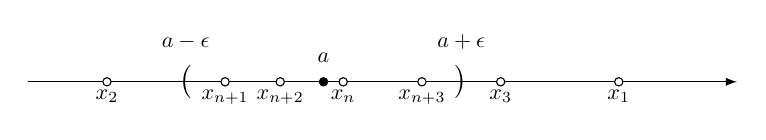
\begin{tikzpicture}
        \draw[-latex] (-4, 0) -- (5, 0);

        \draw[fill=white] (-3, 0) circle (1.5pt) node[below,scale=0.8] {$x_2$};
        \draw[fill=white] (-1.5, 0) circle (1.5pt) node[below,scale=0.8] {$x_{n+1}$};
        \draw[fill=white] (0, 0) circle (1.5pt) node[below,scale=0.8] {$x_n$};
        \draw[fill=white] (2, 0) circle (1.5pt) node[below,scale=0.8] {$x_3$};
        \draw[fill=white] (3.5, 0) circle (1.5pt) node[below,scale=0.8] {$x_1$};
        \draw[fill=white] (-0.8, 0) circle (1.5pt) node[below,scale=0.8] {$x_{n+2}$};
        \draw[fill=white] (1, 0) circle (1.5pt) node[below,scale=0.8] {$x_{n+3}$};

        \draw (-2, 0) node {$ \big( $};
        \draw (-2, 0.5) node[scale=0.8] {$ a-\epsilon $};
        \draw (1.5, 0) node {$ \big) $};
        \draw (1.5, 0.5) node[scale=0.8] {$ a+\epsilon $};

        \draw (-0.25, 0.3) node[scale=0.8] {$ a $};
        \filldraw (-0.25, 0) circle (1.5pt);
    \end{tikzpicture}
\end{figure}

\subsection{无穷小量}\label{subsec:24}
当数列趋向于零时: $x_n\to 0$, 这种情形特别值得注意.

{\kaishu
极限为 $0$ 的数列称为\emph{无穷小量}\index{wuqiongxiao@无穷小量}, 或简称\emph{无穷小}.
}

若在前面数列极限的定义 [\emph{\ref{subsec:23}}] 内使 $a = 0$,
则不等式 \eqref{eq:sequence_limit_definition} 成为
$$
\abs{x_n - 0} = \abs{x_n} < \epsilon \quad (n > N_\epsilon).
$$
这样, 上面无穷小的定义可以不用术语“极限”而更详细地叙述成:
{\kaishu
若数列 $\seqset{x}$ 的绝对值, 自某项起, 成为而且永远保持小于预先指定的任意小的正数 $\epsilon$, 则它称为无穷小.
}

“无穷小”这一历史名称容易引起误解.
除恒等于 $0$ 的平凡情形外, 无穷小数列的某个单独项不能被笼统地称为“很小的量”;
这里描述的是数列的变化过程, 即它的绝对值最终能小于任意预先给定的正数 $\epsilon$.

有了无穷小, 如果设数列 $\seqset{x}$ 以 $a$ 为极限, 则此变量与其极限的差
$$
\alpha_n = x_n - a
$$
显然将为无穷小.

反之, 若 $\alpha_n=x_n-a$ 是无穷小, 则 $x_n \to a$.
因此, $x_n\to a$ 的充分必要条件是差 $\alpha_n=x_n-a$ 为无穷小.
这使我们可以给予“极限”的概念以第二定义:
{\kaishu
若常数 $a$ 与 $x_n$ 的差是无穷小量, 则 $a$ 称为数列 $\seqset{x}$ 的极限.
}

自然而然地, 如果采用极限的第二个定义为极限论的出发点, 则对于无穷小必须应用上述的第二个定义.
否则会产生循环定义: 极限由无穷小确定, 而无穷小又由极限确定.

因此, 若 $x_n \to a$, 则可以表示为
$$
x_n = a + \alpha_n,
$$
式中 $\alpha_n$ 为无穷小.
我们常用这式子以建立数列的极限.

\subsection{例题}\label{subsec:25}
\myrefparagraph{1)}\label{ex:infinitesimal_basic_sequences}
    考察三个数列
    $$
    x_n=\frac{1}{n},\qquad y_n=-\frac{1}{n},\qquad z_n=\frac{(-1)^{n+1}}{n}.
    $$
    它们分别取值为
    $$
    \begin{array}{ccccc}
    \phantom{-}1, & \phantom{-}\dfrac{1}{2}, & \phantom{-}\dfrac{1}{3}, & \phantom{-}\dfrac{1}{4}, & \cdots \\[0.8em]
    -1, & -\dfrac{1}{2}, & -\dfrac{1}{3}, & -\dfrac{1}{4}, & \cdots \\[0.8em]
    \phantom{-}1, & -\dfrac{1}{2}, & \phantom{-}\dfrac{1}{3}, & -\dfrac{1}{4}, & \cdots
    \end{array}
    $$
    要证明这三个数列都是无穷小.

    观察到它们的绝对值都等于 $\dfrac{1}{n}$, 因此当 $n>\dfrac{1}{\epsilon}$ 时, 便有
    $$
    \abs{x_n}<\epsilon,\qquad \abs{y_n}<\epsilon,\qquad \abs{z_n}<\epsilon.
    $$
    这样, 我们取 $\dfrac{1}{\epsilon}$ 的整数部分,
    令 $N_\epsilon = \max\left\{1,\floor{\dfrac{1}{\epsilon}}\right\}$
    \footnote{$\max\{\cdots\}$ 指在所给数中选择最大的那个数,
    但实际情况是 $\epsilon$ 常常是个非常小的数, $\dfrac{1}{\epsilon}$ 将会远远大于 1,
    所以也可以将 $\max$ 省略只保留 $N_\epsilon = \floor{\dfrac{1}{\epsilon}}$; $\floor{p}$ 表示不超过 $p$ 的最大整数, 或简称数 $p$ 的整数部分.},
    就完成了证明.

    注意到第一个变量常大于其极限 0, 第二个常小于 0, 第三个则交迭地忽大于忽小于 0,
    尽管如此, 这都不影响其最终极限为 $0$.

\myrefparagraph{2)}\label{ex:oscillatory_zero_limit}
    若设
    $$
    x_n=\frac{2+(-1)^n}{n}.
    $$
    则数列为
    $$
    1,\ \frac{3}{2},\ \frac{1}{3},\ \frac{3}{4},\ \frac{1}{5},\ \frac{3}{6},\ \ldots.
    $$
    它一会儿靠近 $0$, 一会儿又离开一些, 但仍有
    $$
    \abs{x_n}\leq \frac{3}{n}<\epsilon,
    \qquad
    \text{当 } \ n>\max\left\{1,\floor{\frac{3}{\epsilon}}\right\}\text{ 时}.
    $$
    因而 $x_n\to0$.

\myrefparagraph{3)}\label{ex:zero_odd_terms_limit}
    设
    $$
    x_n=\frac{1+(-1)^n}{n}.
    $$
    这里所有奇数项都等于 $0$, 偶数项为 $2/n$. 由于
    $$
    \abs{x_n}\leq\frac{2}{n}<\epsilon,
    \qquad\text{当 } \ n>\max\left\{1,\floor{\frac{2}{\epsilon}}\right\}\text{ 时},
    $$
    所以 $x_n\to0$.
    数列可以在无穷多个位置恰好取到极限值, 这同样不妨碍极限的存在.

    \ref{ex:infinitesimal_basic_sequences}、 \ref{ex:oscillatory_zero_limit}、 \ref{ex:zero_odd_terms_limit}
    这些简单的例子是很有趣的, 它们体现了数列在趋于极限的方式上的各种可能性.
    无论是变量的值是否均在极限值的一方;
    还是变量是否每一步都向其极限接近;
    又或是变量是否能达到其极限, 即是否具有等于极限的数值;
    这些都不关紧要.
    重要的仅是定义中所说的:
    变量在最后, 即项数充分远时的数值, 与极限值之差要是任意小.
\myrefparagraph{4)}\label{ex:rational_sequence_one_third}
    再来看看更为复杂的例子.
    设
    $$
    x_n=\frac{n^2-n+2}{3n^2+2n-4}.
    $$
    证明 $x_n\to\dfrac{1}{3}$.

    为此直接比较 $x_n$ 与候选极限, 当 $n>2$ 时,
    $$
    x_n-\frac{1}{3}
    =\frac{-5n+10}{3(3n^2+2n-4)}
    $$
    估计其绝对值, 当 $n>2$ 时有
    $$
    \abs{x_n-\frac{1}{3}}
    =\frac{5n-10}{3(3n^2+2n-4)}
    <\frac{5n}{3(3n^2-4)}
    <\frac{5n}{3\cdot2n^2}<\frac{1}{n}.
    $$
    因此取
    $$
    N_\epsilon=\max\left\{2,\floor{\frac{1}{\epsilon}}\right\},
    $$
    这式的结果便小于 $\epsilon$, 这就证明了 $x_n\to\dfrac{1}{3}$.

\myrefparagraph{5)}\label{ex:nth_root_constant_supplement}
    对 $a>1$, 数列
    $$
    x_n=a^{\frac{1}{n}}=\sqrt[n]{a}
    $$
    要证 $x_n\to1$.
    若应用绪论中的 Bernoulli 不等式 \eqref{eq:bernoulli_application}, 则有
    $$
    \abs{x_n-1} = \sqrt[n]{a} - 1 \leq \frac{a-1}{n} < \epsilon,
    \quad \text{当} \ n > N_\epsilon = \max\left\{1,\floor{\dfrac{a-1}{\epsilon}}\right\}.
    $$
    亦可以直接运用对数
    $$
    \abs{x_n-1} = \sqrt[n]{a} - 1 < \epsilon
    \quad\Longleftrightarrow\quad
    \frac{1}{n} < \log_a(1+\epsilon).
    $$
    因此也可以取
    $$
    N_\epsilon=\max\left\{1,\floor{\frac{1}{\log_a(1+\epsilon)}}\right\}.
    $$

    由于所选的方法不同, 我们便得出不同的 $N_\epsilon$ 的表达.
    例如, 在 $ a = 10, \epsilon = 0.01 $ 时, 依第一种方法得
    $
    N_{0.01} = \dfrac{9}{0.01} = 900,
    $
    而依第二种方法得
    $
    N_{0.01} = \floor{\dfrac{1}{0.004 \ 32 \ \cdots}} = 231.
    $
    注意到
    $
    10^{\frac{1}{231}} = 1.010 \, 017 \, \cdots
    $
    与 $1$ 的差已大于 $\varepsilon = 0.01$,
    所以依第二种方法我们得到的 \( N_{0.01}=231 \) 是一切可能的数值中的最小者,
    也就是说为了满足 $ a = 10, \epsilon = 0.01 $ 的条件, 我们的 $N_{0.01}$ 最小只能到 231.
    这在一般情形也是如此, 因为很容易看出, 当
    $
    n \leq \dfrac{1}{\log_a(1 + \varepsilon)}
    $
    时必有
    $
    a^{\frac{1}{n}} - 1 \geq \varepsilon.
    $

    注意: 如果只是要证明极限存在,
    那么我们其实并不需要关心 \( N_\varepsilon \) 最小可能的数值.
    只需保证不等式 \eqref{eq:sequence_limit_definition} 能成立就好了,
    至于从哪一项开始, 位置远些或近些, 可以不必管它.

\myrefparagraph{6)}\label{ex:geometric_infinitesimal}
    若 $\abs{q}<1$, 则数列
    $$
    a_n=q^n
    $$
    是无穷小.

    $q=0$ 时结论显然;
    若 $0<\abs{q}<1$, 证明时只需考虑 $0<\epsilon<1$, 此时
    $$
    \abs{a_n}=\abs{q}^n<\epsilon, \qquad \text{当} \ n>\frac{\ln\epsilon}{\ln\abs{q}} \text{时}.
    $$
    更一般地, 任意常数 $A$ 的数列 $Aq^n$ 也趋于 $0$.

\myrefparagraph{7)}\label{ex:geometric_series_sum}
    再考察无穷等比级数
    $$
    a+aq+aq^2+\cdots+aq^{n-1}+\cdots,\qquad \abs{q}<1.
    $$
    它的前 $n$ 项和为
    $$
    s_n=\frac{a-aq^n}{1-q}=\frac{a}{1-q}-\frac{a}{1-q}q^n.
    $$
    而 $q^n\to0$, 于是它们的和
    $$
    s = \lim_{n\to\infty}s_n=\frac{a}{1-q}.
    $$

\myrefparagraph{8)}\label{ex:averaging_recurrence_limit}
    给定 $x_0=a$、$x_1=b$, 并令
    $$
    x_n=\frac{x_{n-2}+x_{n-1}}{2}\qquad(n\geq2).
    $$
    为了考察这个数列的极限,
    我们将两边同时减去 $x_{n-1}$, 有
    $$
    x_n-x_{n-1}=-\frac{1}{2}(x_{n-1}-x_{n-2}).
    $$
    因而
    $$
    x_n-x_{n-1}=\left(-\frac{1}{2}\right)^{n-1}(b-a),
    $$
    进而
    $$
    x_n=a+(b-a)\sum_{k=0}^{n-1}\left(-\frac{1}{2}\right)^k\qquad(n\geq1).
    $$
    利用等比级数的求和公式, 得到
    $$
    \lim_{n\to\infty}x_n=a+\frac{2}{3}(b-a)=\frac{a+2b}{3}.
    $$

\myrefparagraph{9)}\label{ex:series_partial_sums}
    与等比数列相似, 给定一般数列 $\{a_n\}$, 将它们依次相加, 做成“部分和”
    $$
    A_1 = a_1, \ A_2 = a_1+a_2,\ \cdots,\ A_n=a_1+a_2+\cdots+a_n,\ \cdots
    $$
    若 $A_n\to A$, 就把 $A$ 定义为
    $$
    a_1+a_2+\cdots+a_n+\cdots
    $$
    的和, 上面这个式子也被称为\emph{无穷级数}\index{wuqiongjishu@无穷级数}.
    这时称该级数为\emph{收敛级数}.
    例如
    $$
    \frac{1}{1\cdot2}+\frac{1}{2\cdot3}+\frac{1}{3\cdot4}+\cdots
    $$
    的第 $n$ 个部分和为
    \footnote{$\displaystyle \sum_{k=1}^n a_k$ 是对求和式 $a_1 + a_2 + \cdots + a_n$ 的简写.}
    $$
    A_n=\sum_{k=1}^n\frac{1}{k(k+1)}
    =\sum_{k=1}^n\left(\frac{1}{k}-\frac{1}{k+1}\right)
    =1-\frac{1}{n+1}\to1.
    $$
    因而该级数的和为 $1$.

    \enlargethispage{0.5\baselineskip}
    相反, 如果级数没有有限和, 这时我们就说这个级数\emph{发散}.
    例如
    $$1+1+1+\cdots$$
    就是这样的级数.

\subsection{关于有极限数列的一些定理}\label{subsec:26}
设数列 $\seqset{x}$ 有极限 $a$, 那么由极限定义可知, 对任意 $\epsilon>0$, 从某一项开始都有不等式 \eqref{eq:limit_inequality}:
$$
a - \epsilon < x_n < a + \epsilon,
$$
这一估计可以用来比较数列的后续各项与任意给定常数的大小.
若有数 $p<a$（或 $q>a$）,
都可以选取 $\epsilon<a-p$（或 $\epsilon<q-a$）, 并找到序号 $N$, 使当 $n>N$ 时有
$$
x_n>a-\epsilon > p \qquad \text{（或 }\ x_n<a+\epsilon<q\text{）}.
$$
这样我们就证明了

\myrefparagraph{1\textdegree}\label{prop:eventual_order_from_limit}
{\kaishu 若 $x_n\to a$, 且 $a>p$（或 $a<q$）, 则从某一项开始, 必有
$$
x_n>p \qquad \text{（或 }\ x_n<q\text{）}.
$$}

这一个简单的命题包含一系列有用的推论.

\myrefparagraph{2\textdegree}\label{prop:eventual_sign_preservation}
{\kaishu 若 $x_n\to a$, 且 $a>0$（或 $a<0$）, 则从某一项开始, 必有
$$
x_n>0 \qquad \text{（或 }\ x_n<0\text{）}.
$$}

这被称为收敛数列的\emph{保号性}\index{baohaoxing@保号性}.
它是命题 \ref{prop:eventual_order_from_limit} 在 $p=0$（或 $q=0$）时的直接推论.
更为一般的结果是:
\myrefparagraph{3\textdegree}\label{prop:convergent_sequence_away_from_zero}
{\kaishu 若 $x_n\to a$, 且 $a\neq0$, 则存在正数 $r$ 和自然数 $N$, 使当 $n>N$ 时,
$$
\abs{x_n}>r>0.
$$}

事实上, 当 $a>0 \ (<0)$ 时, 可以取
$$0<p<a \ (a<q<0),$$
再假定 $r=p\ (r=\abs{q})$,
应用命题 \ref{prop:eventual_order_from_limit} 即可.

\myrefparagraph{4\textdegree}\label{prop:convergent_sequence_bounded}
{\kaishu 若数列 $\seqset{x}$ 有有限极限 $a$, 则它必为有界数列, 即存在常数 $M>0$, 使
$$
\abs{x_n}\leq M \qquad (n=1,2,\cdots).
$$}

\enlargethispage{0.5\baselineskip}
取 $M'>\abs{a}$. 由命题 \ref{prop:eventual_order_from_limit}, 存在 $N$, 使当 $n>N$ 时,
$$
-M'<x_n<M',\quad\text{即}\quad \abs{x_n}<M'.
$$
这不等式只可能对于数列的前 $N$ 项(或它们之中的某几项)不满足.
因此只需再令
$$
M=\max\bbbrac{\abs{x_1},\abs{x_2},\ldots,\abs{x_N},M'},
$$
便有 $\abs{x_n}\leq M$ 对一切自然数 $n$ 成立.

\begin{remark}
\myrefparagraph{I.}\label{note:bounded_sequence_equivalent_definition}
数列 $\seqset{x}$ 有界, 也可以等价地写成: 存在两个有限数 $k,g$, 使
$$
k\leq x_n\leq g \qquad (n=1,2,\ldots).
$$
若已知这组不等式, 取 $M=\max\bbbrac{\abs{k},\abs{g}}$, 便有 $\abs{x_n}\leq M$; 反过来, 由 $\abs{x_n}\leq M$ 可得 $-M\leq x_n\leq M$.

\myrefparagraph{II.}\label{note:bounded_not_necessarily_convergent}
命题 \ref{prop:convergent_sequence_bounded} 的逆命题不成立: 有界数列未必收敛. 例如
$$
x_n=(-1)^{n+1}
$$
恒有 $\abs{x_n}=1$, 但它在 $1$ 与 $-1$ 之间交替取值, 没有极限.
\end{remark}

最后可以根据命题 \ref{prop:eventual_order_from_limit} 证明极限的\emph{唯一性}.
\myrefparagraph{5\textdegree}\label{prop:limit_uniqueness}
{\kaishu 数列的极限若存在, 则必定唯一\index{jixiandeweiyixing@极限的唯一性};
也就是说, 一个数列不能同时趋于两个相异的极限. }

用反证法证明. 假设同时有 $x_n\to a$ 和 $x_n\to b$, 并且 $a<b$. 在 $a$ 与 $b$ 之间任取一数 $r$, 使
$$
a<r<b.
$$
由命题 \ref{prop:eventual_order_from_limit}, 存在 $N'$, 使当 $n>N'$ 时有 $x_n<r$; 又存在 $N''$, 使当 $n>N''$ 时有 $x_n>r$. 于是当
$$
n>\max\bbbrac{N',N''}
$$
时, $x_n$ 将同时满足 $x_n<r$ 和 $x_n>r$, 这个矛盾便证明了我们的命题.

\subsection{无穷大量}\label{subsec:27}
\emph{无穷大量}\index{wuqiongdaliang@无穷大量}(或简称\emph{无穷大}),
在某种意义上是与无穷小量相反的量.

{\kaishu
若数列 $\{x_n\}$ 从某项开始, 其绝对值都将大于预先指定的任意大数 $E > 0$,
$$
\abs{x_n} > E \quad (\text{当} \ n > N_E \ \text{时}),
$$
$\seqset{x}$ 便称为无穷大.}

如同无穷小的情形, 所谓“无穷大”, 说的是数列变化的过程, 而不是某一项的数值,
无穷大量中任一个别数值都不能当作“大量”来看待.

最简单的例子是
$$
x_n=n,\quad y_n=-n,\quad z_n=(-1)^{n+1}n.
$$
它们在取定
$
N_E=\floor{E}
$
后, 都能使各自的绝对值大于事先指定的数 $E$.

进一步地可以发现, $\seqset{x}$ 在变化过程中始终带正号,
$\seqset{y}$ 始终带负号, $\seqset{z}$ 则是正负交替出现.
前两种情形可以进一步说明:
{\kaishu 若数列 $\seqset{x}$ 是无穷大量, 并且从某项开始保持一定的符号(+或−),
则按照符号的正或负, 我们说 $\seqset{x}$ 有极限 $+\infty$ 或 $-\infty$, 并写成:
$$
\limto{n}x_n=+\infty,\quad x_n\to+\infty
\qquad\text{或}\qquad
\limto{n}x_n=-\infty,\quad x_n\to-\infty.
$$}
在这两种情形中, 可以分别用不等式
$$
x_n>E \quad\text{或}\quad x_n<-E
$$
来代替 $\abs{x_n}>E$, 作为带确定符号的无穷极限的定义.
一般的无穷大量则统一写成
$$
\abs{x_n}\to+\infty.
$$

因此, 前面例子里的 $\{x_n\}$ 趋向 $+\infty$, $\{y_n\}$ 趋向 $-\infty$.
至于 $\{z_n\}$, 它没有有限极限, 也不趋向 $+\infty$ 或 $-\infty$;
但由于 $\abs{z_n}\to+\infty$, 它仍是一般意义下的无穷大量.

关于这些“广义的数” $\pm\infty$, 我们在 \emph{\ref{subsec:11}} 已讨论过,
它们必须结合上述定义使用, 不能不加条件地当作普通实数进行四则运算.
按照习惯, 语境明确时常用 $\infty$ 代替 $+\infty$.

再看一个无穷大量的例子:
$$
x_n=Q^n,\qquad \abs{Q}>1.
$$
任给 $E>0$, 要使 $\abs{x_n}=\abs{Q}^n>E$, 只需
$$
n\ln\abs{Q}>\ln E, \quad \text{即} \ n>\frac{\ln E}{\ln\abs{Q}}.
$$
因此取
$$
N_E=\max\left\{1,\floor{\frac{\ln E}{\ln\abs{Q}}}\right\}
$$
就证明了我们的命题
\footnote{这里取最大值是为了保证当 $0<E<1$ 时, $N_E$ 仍是正整数.}.
因此, 当 $\abs{Q}>1$ 时, $Q^n$ 是无穷大量.
同样, 当 $Q>1$ 时有 $Q^n\to+\infty$;
当 $Q<-1$ 时, $Q^n$ 的绝对值趋于 $+\infty$, 但它本身没有带符号的无穷极限.

最后, 讲一讲无穷大量与无穷小量间的简单关系:

{\kaishu
若 $\seqset{x}$ 是无穷大量, 则从某项开始必有 $x_n\neq0$.
从这一项起令 $\alpha_n=\dfrac{1}{x_n}$, 并任意补定有限个初始项, 所得数列 $\seqset{\alpha}$ 是无穷小.
}
\begin{proof}
取任意数 $\epsilon>0$. 因 $\abs{x_n}\to+\infty$, 故对于数 $E=\dfrac{1}{\epsilon}$ 可以求得序号 $N$, 使
$$
\abs{x_n}>\frac{1}{\epsilon}\qquad(n>N).
$$
于是对于这样的 $n$, 有
$$
\abs{\alpha_n} = \abs{\frac{1}{x_n}} < \epsilon,
$$
这就证明了我们的命题.
\end{proof}

仿此, 可以证明逆命题:

{\kaishu
若无穷小数列 $\seqset{\alpha}$ 的各项均不为 $0$, 则其倒数 $x_n=\dfrac{1}{\alpha_n}$ 是无穷大量.
}

\begin{remark}
引入无穷极限并不会破坏命题 \ref{prop:limit_uniqueness} 中建立的极限的唯一性.
由命题 \ref{prop:convergent_sequence_bounded}, 有有限极限的数列必定有界;
与之相反的, 我们可以建立无界的概念:

若不存在常数 $M>0$, 使 $\abs{x_n}\leq M$ 对一切自然数 $n$ 成立,
就称数列 $\seqset{x}$ \emph{无界}\index{wujieshulie@无界数列}.
这等价于:
{\kaishu 任给 $E>0$ 和自然数 $N$, 总能找到某个 $n>N$, 使
$$
\abs{x_n}>E.
$$}
很明显看出, 无穷大量一定是无界的.
因此, 一个数列不可能既有有限极限, 又趋于无穷.

但是无界数列与无穷大却不是等价的,
最关键的点在于无界数列中的序号 $n$ 可以随 $E$ 和 $N$ 改变,
并不要求从某项开始, 所有项的绝对值都大于 $E$.
例如, 数列
$$
x_n=\begin{cases}
    n, & n\text{ 为偶数},\\
    0, & n\text{ 为奇数}
\end{cases}
$$
是无界的, 因为它的偶数项可以任意大;
但它含有无穷多个等于 $0$ 的项, 因而并不趋于无穷.

这说明“无界”比“无穷大”弱.
换言之, {\kaishu 无穷大量一定无界, 但无界数列未必是无穷大量. }
\end{remark}

\begin{comment}
\section{极限的定理·若干容易求得的极限}
\subsection{比较性} {\kaishu 若两个数列 $\seqset{x} , \seqset{y}$ 对应项常满足不等式 $x_n \geq y_n$, 并且各趋于有限极限:
$$
\limto{n} x_n = a, \quad \limto{n} y_n = b,
$$
则必 $a \geq b$.}

假定是相反的情形: 设 $a < b$.
任取在 $a$ 与 $b$ 间的一数 $r$, $a < r < b$.
那么, 一方面, 可以求得序号 $N'$, 使当 $n > N'$ 时成立 $x_n < r$;
另一方面, 又可求得序号 $N''$, 使当 $n > N''$ 时成立 $y_n > r$.
若 $N$ 大于 $N'$ 和 $N''$, 则当 $n > N$ 时将同时成立不等式
$$
x_n < r, \quad y_n > r \Rightarrow x_n < y_n,
$$
这与假定矛盾.

比较性使得我们得以对不等式(连同着等号的)取极限: 由 $x_n \geq y_n$ 得结论:
$$
\limto{n} x_n \geq \limto{n} y_n.
$$
当然, 各处的 $\geq$ 号都可以换成 $\leq$ 号.

请注意, 由严格的不等式 $x_n > y_n$, 一般说来, 不能推得严格的不等式 $\displaystyle \limto{n} x_n > \limto{n} y_n$, 而仅能推得: $\displaystyle \limto{n} x_n \geqslant \limto{n} y_n$.

例如, 对于一切的自然数 $n$, 都有 $\displaystyle \frac{1}{n} > -\frac{1}{n}$, 但
$$
\limto{n} \frac{1}{n} = \limto{n} \brac{-\frac{1}{n}} = 0.
$$
最后的极限并不是严格大于.

\subsection{夹逼准则}
{\kaishu 若 $x_n, y_n, z_n$ 恒满足不等式
$$
x_n \leqslant y_n \leqslant z_n,
$$
并且 $x_n$ 及 $z_n$ 趋向同一极限 $a$:
$$
\limto{n} x_n = \limto{n} z_n = a,
$$
则 $y_n$ 亦必以 $a$ 为极限:
$$
\limto{n} y_n = a.
$$}

指定任意的 $\epsilon > 0$. 对于这 $\epsilon$, 首先可以求得序号 $N'$, 使当 $n > N'$ 时
$$
a - \epsilon < x_n < a + \epsilon.
$$
其次, 又可求得序号 $N''$, 使当 $n > N''$ 时
$$
a - \epsilon < z_n < a + \epsilon.
$$
设 $N$ 大于 $N'$ 及 $N''$, 则当 $n > N$ 时, 上述两不等式都能满足, 故
$$
a - \epsilon < x_n \leqslant y_n \leqslant z_n < a + \epsilon.
$$
结果当 $n > N$ 时
$$
a - \epsilon < y_n < a + \epsilon \quad \text{或} \quad \abs{y_n - a} < \epsilon.
$$
这样, 实际上就是 $\displaystyle \limto{n} y_n = a$.

\subsection{无穷小引理}
在后面极限的中我们将要同时考虑两个(或更多个)数列极限, 并在它们之间施行算术运算.
在证明关于极限的算术运算的性质时, 下面两个关于无穷小的引理, 将担任着重要的角色.

\begin{lemma} \label{n0}
    任何有限个无穷小的和亦是无穷小量.
\end{lemma}

\begin{proof}
我们只证明对于二无穷小 $\alpha_n$ 及 $\beta_n$ 的情形(一般的情形仿此讨论).

给定任意的 $\epsilon > 0$.
根据无穷小的定义, 由 $\epsilon$ 可以决定无穷小 $\alpha_n$ 的序号 $N'$, 以及关于 $\beta_n$ 的序号 $N''$, 使当 $n > N', N''$ 时有
$$
\abs{\alpha_n} < \frac{\epsilon}{2}, \quad \abs{\beta_n} < \frac{\epsilon}{2}.
$$
若取自然数 $N$ 大于 $N'$ 及 $N''$, 则当 $n > N$ 时, 两不等式同时成立, 这样, 便有
$$
\abs{\alpha_n + \beta_n} \leqslant \abs{\alpha_n} + \abs{\beta_n} < \frac{\epsilon}{2} + \frac{\epsilon}{2} = \epsilon.
$$
因此, $\alpha_n + \beta_n$ 也是无穷小.
\end{proof}

\begin{lemma} \label{a0}
    有界变量 $x_n$ 与无穷小 $\alpha_n$ 的乘积仍是无穷小.
\end{lemma}

\begin{proof}
设对于一切 $n$ 有
$$
\abs{x_n} \leqslant M \quad (M > 0).
$$
若给定任意数 $\epsilon > 0$, 则依 $\dfrac{\epsilon}{M}$, 对于无穷小 $\alpha_n$ 可以求出 $N$, 使当 $n > N$ 时有
$$
\abs{\alpha_n} < \frac{\epsilon}{M}.
$$
对于这种 $n$, 显然有
$$
\abs{x_n \cdot \alpha_n} = \abs{x_n} \cdot \abs{\alpha_n} < M \cdot \frac{\epsilon}{M} = \epsilon.
$$
由此推得, $x_n \cdot \alpha_n$ 为无穷小.
\end{proof}

\subsection{四则运算}
有了上述两个引理, 我们便可以叙述极限的四则运算, 有了它们便可以不必把一切与极限有关的问题都追溯到“极限”的定义, 然后依指定的 $\epsilon$ 找出对应的 $N$ 等等, 使得极限的计算将大为简化.

1\textdegree~
{\kaishu 若数列 $\{x_n\}$ 及 $\{y_n\}$ 趋于有限极限:
$$
\limto{n} x_n = a, \quad \limto{n} y_n = b,
$$
则它们的和(差)仍趋于有限极限, 并且
$$
\limto{n} \brac{x_n \pm y_n} = a \pm b.
$$}

由极限的第二定义, 推得
$$
x_n = a + \alpha_n, \quad y_n = b + \beta_n
$$
式中 $\alpha_n$ 及 $\beta_n$ 为无穷小. 故
$$
x_n \pm y_n = (a \pm b) + (\alpha_n \pm \beta_n).
$$
这里的 $\alpha_n \pm \beta_n$ 依引理 \ref{n0} 为无穷小.
因此, 应用极限的第二定义, 可以证明 $x_n \pm y_n$ 有极限 $a \pm b$.

这定理及其证法, 可以推广到任意有限个有极限的数列相加的情形.

2\textdegree~
{\kaishu 若数列 $\{x_n\}$ 及 $\{y_n\}$ 趋于有限极限:
$$
\limto{n} x_n = a, \quad \limto{n} y_n = b,
$$
则它们的积仍趋于有限极限, 并且
$$
\limto{n} x_n y_n = ab.
$$}

仍由极限的第二定义, 这次便有
$$
x_n y_n = ab + (a\beta_n + b\alpha_n + \alpha_n\beta_n).
$$
依引理 \ref{n0} 及 \ref{a0}, 在括号内的式子为无穷小量.由此便推得, $x_n y_n$ 确趋于极限 $ab$.

这定理同样可以推广到任意有限个有极限的数列相乘的情形.

3\textdegree~
{\kaishu 若数列 $\{x_n\}$ 及 $\{y_n\}$ 趋于有限极限:
$$
\limto{n} x_n = a, \quad \limto{n} y_n = b,
$$
并且 $b$ \emph{异于} 0, 则它们的比仍趋于有限极限, 并且
$$
\limto{n} \frac{x_n}{y_n} = \frac{a}{b}.
$$}

由于 $b \neq 0$, 根据保号性, 由某项开始, 不仅 $y_n \neq 0$, 且有
$$
\abs{y_n} > r > 0,
$$
式中 $r$ 是常数.
对于使上面的不等式成立的那些 $n$, 比 $\dfrac{x_n}{y_n}$ 显然是有意义的.

依旧从极限的第二定义出发, 得
$$
\frac{x_n}{y_n} - \frac{a}{b} = \frac{a + \alpha_n}{b + \beta_n} - \frac{a}{b} = \frac{1}{by_n}(b\alpha_n - a\beta_n).
$$

依引理 \ref{n0} 及 \ref{a0}, 在括号内的式子 $b\alpha_n - a\beta_n$ 为无穷小量.
根据开始时的叙述, 而其乘数将是有界变量:
$$
\abs{\frac{1}{by_n}} = \frac{1}{\abs{b}\abs{y_n}} < \frac{1}{\abs{b}r}.
$$
因此, 依引理 \ref{a0}, 等式右边的积将是无穷小.
但它表示 $\dfrac{x_n}{y_n}$ 及数 $\dfrac{a}{b}$ 的差, 故 $\dfrac{x_n}{y_n}$ 的极限是 $\dfrac{a}{b}$.
此即所要证的.

\subsection{未定式}
上面我们讨论了
$$
x_n \pm y_n, \quad x_ny_n, \quad \frac{x_n}{y_n},
$$
并在 $\seqset{x}$ 及 $\seqset{y}$ 都趋于有限极限的假定下在相除的情形, $\seqset{y}$ 的极限应不等于零, 各式子的极限.

今再详述余下的尚未考虑的情形, 当 $\seqset{x}$ 及 $\seqset{y}$ (其中之一或两者) 的极限是无穷大时, 或(若论及除法)当分母的极限为零时.
由这两种情形, 这里讲述四种重要而且有用的未定式.

1\textdegree~
我们首先来看商 $\dfrac{x_n}{y_n}$, 设 $\seqset{x}$ 及 $\seqset{y}$ 同时趋于零.
下面给出三种情况:

设 $x_n = \dfrac{1}{n^2}, y_n = \dfrac{1}{n}$, 则两数列各自趋于零, 它们的比 $\dfrac{x_n}{y_n} = \dfrac{1}{n}$ 也趋于零; 反之, 设 $x_n = \dfrac{1}{n}, y_n = \dfrac{1}{n^2}$, 虽然它们依旧各自趋于零, 但这次它们的比 $\dfrac{x_n}{y_n} = n$ 趋于 $\infty$.

再取任一异于零的数 $a$, 并作出两个无穷小 $x_n = \dfrac{a}{n}$ 及 $y_n = \dfrac{1}{n}$ 便知它们的比有极限为 $a$.

最后, 若 $x_n = \dfrac{(-1)^{n+1}}{n}, y_n = \dfrac{1}{n}$ (两者各有极限为零), 则比 $\dfrac{x_n}{y_n} = (-1)^{n+1}$ 没有极限.

这样, 单知道 $\seqset{x}$ 及 $\seqset{y}$ 的极限 0, 在目前的情形下我们无法判断它们的比的极限, 必须知道数列本身改变的规律, 并直接研究比 $\dfrac{x_n}{y_n}$.
为了要表达当 $x_n \to 0$ 及 $y_n \to 0$ 的情形时的未定性, 就说, {\kaishu 表达式 $\dfrac{x_n}{y_n}$ 是 $\dfrac{0}{0}$ 型的未定式}.

2\textdegree~
在同时 $x_n \to \pm \infty$ 及 $y_n \to \pm \infty$ 的情形, 亦有类似的情况.
若不知数列本身, 关于它们的比的极限便不能作出一般的论断.
这一事实可以用完全类似于 1\textdegree 内引用的那些例题来表明:
\begin{align*}
    &x_n = n \to \infty, \quad y_n = n^2 \to \infty, \quad \frac{x_n}{y_n} = \frac{1}{n} \to 0; \\
    &x_n = n^2 \to \infty, \quad y_n = n \to \infty, \quad \frac{x_n}{y_n} = n \to \infty; \\
    &x_n = an \to \pm \infty \quad (a \neq 0), \quad y_n = n \to \infty, \quad \frac{x_n}{y_n} = a \to a; \\
    &x_n = [2 + (-1)^{n+1}]n \to \infty, \quad y_n = n \to \infty, \quad \frac{x_n}{y_n} = 2 + (-1)^{n+1} \ \text{发散}
\end{align*}

在这种情况下, 就说, {\kaishu 表达式 $\dfrac{x_n}{y_n}$ 是 $\dfrac{\infty}{\infty}$ 型的未定式}.

3\textdegree~
若 $\seqset{x}$ 趋于零, 同时 $\seqset{y}$ 趋于 $\pm \infty$, 则研究积 $x_n y_n$ 的极限时, 我们又遇到像 1\textdegree 及 2\textdegree 内所遇到的那种未定性. 关于这点可以由下面的例题证实它:
\begin{align*}
    &x_n = \frac{1}{n^2} \to 0, \quad y_n = n \to \infty, \quad x_n y_n = \frac{1}{n} \to 0; \\
    &x_n = \frac{1}{n} \to 0, \quad y_n = n^2 \to \infty, \quad x_n y_n = n \to \infty; \\
    &x_n = \frac{a}{n} \to 0 \quad (a \neq 0), \quad y_n = n \to \infty, \quad x_n y_n = a \to a; \\
    &x_n = \frac{(-1)^{n+1}}{n} \to 0, \quad y_n = n \to \infty, \quad x_n y_n = (-1)^{n+1} \ \text{发散}
\end{align*}

在这种情况下, 就说, {\kaishu 表达式 $x_n y_n$ 是 $0 \cdot \infty$ 型的未定式}.

4\textdegree~
这里讲当 $\seqset{x}$ 及 $\seqset{y}$ 趋于异号的无穷大时, 若不知道 $x_n$ 及 $y_n$ 本身, 也不可能确定 $x_n + y_n$ 的极限. 在这里所表示的各种不同的可能性可用下面的例题表明它:
\begin{align*}
    &x_n = 2n \to +\infty, \quad y_n = -n \to -\infty, \quad x_n + y_n = n \to +\infty; \\
    &x_n = n \to +\infty, \quad y_n = -2n \to -\infty, \quad x_n + y_n = -n \to -\infty; \\
    &x_n = n + a \to +\infty, \quad y_n = -n \to -\infty, \quad x_n + y_n = a \to a; \\
    &x_n = n + (-1)^{n+1} \to +\infty, \quad y_n = -n \to -\infty, \quad x_n + y_n = (-1)^{n+1} \ \text{发散}
\end{align*}

因此, 当 $x_n \to +\infty$ 及 $y_n \to -\infty$ 时, 即说, {\kaishu 表达式 $x_n + y_n$ 是 $\infty - \infty$ 型的未定式}.

综合上面所讨论, 当提出了依 $\seqset{x}$ 及 $\seqset{y}$ 的极限去确定由它们所组成的四则运算的极限这个问题以后, 我们可以发现不可能解答的四种情形: 即型为
$$
\frac{0}{0}, \quad \frac{\infty}{\infty}, \quad 0 \cdot \infty, \quad \infty - \infty
$$
的\emph{未定式}.在这些情形, 必须注意数列 $\seqset{x}$ 及 $\seqset{y}$ 的改变规律, 直接去研究我们所关心的式子.
类似的研究称为\emph{未定式的定值法}.
以后它并不永远像上面所举的例题那样简单.

将已给式子\emph{变形}以消除其“未定性”是未定式定值法中常用的方法.

\begin{example}
    考察这么一个极限, 设 $p(n)$ 是整数 $n$ 的常系数多项式:
    $$
    p(n) = a_0n^k + a_1n^{k-1} + \cdots + a_{k-1}n + a_k,
    $$
    若这多项式的一切系数全是正(负)的, 则显然 $p(n)$ 的极限是 $+\infty$ ($-\infty$).
    但在系数为异号的情形, 某些项趋向 $+\infty$, 另一些项趋向 $-\infty$, 就遇到 $\infty - \infty$ 型的未定式.

    要确定这一未定式, 可以把 $p(n)$ 写成
    $$
    p(n) = n^k \brac{a_0 + \frac{a_1}{n} + \cdots + \frac{a_{k-1}}{n^{k-1}} + \frac{a_k}{n^k}}.
    $$
    因为在括号内的一切加数, 从第二项起, 当 $n$ 增大时为无穷小, 所以括号内的式子有极限为 $a_0$.
    第一个乘数趋向 $+\infty$. 则整个式子趋于 $+\infty$ 或 $-\infty$, 结果视 $a_0$ 的符号而定.
\end{example}

\begin{example}
    若 $q(n)$ 也是多项式:
    $$q(n) = b_0n^l + b_1n^{l-1} + \cdots + b_{l-1}n + b_l, $$
    则商 $\dfrac{p(n)}{q(n)}$ 在 $n\to\infty$ 时是 $\dfrac{\infty}{\infty}$ 型的未定式.

    在这里也就将每一个多项式变形, 如同在上例内做过的那样, 则得:
    $$
    \frac{p(n)}{q(n)} = n^{k-l} \frac{a_0 + \dfrac{a_1}{n} + \cdots + \dfrac{a_k}{n^k}}{b_0 + \dfrac{b_1}{n} + \cdots + \dfrac{b_l}{n^l}}.
    $$
    上式右边第二个乘数有一有限极限 $\dfrac{a_0}{b_0}$.
    若两个多项式的幂次相等: $k = l$, 则比 $\dfrac{p(n)}{q(n)}$ 的极限为 $\dfrac{a_0}{b_0}$.
    当 $k > l$ 时, 第一个乘数趋向 $\infty$, 故所考察的比亦趋向 $\pm\infty$ (其符号视 $\dfrac{a_0}{b_0}$ 的符号而定).
    最后, 当 $k < l$ 时, 第一个乘数趋向零, 于是整个式子跟着它趋向零.
\end{example}

\begin{example}
    证明, 在 $0 < k < 1$ 时,
    $$
    \limto{n} [(n+1)^k - n^k] = 0.
    $$

    这里是 $\infty - \infty$ 型的未定式.
    进行变形:
    $$
    0 < (n+1)^k - n^k = n^k \bbrac{\brac{1 + \frac{1}{n}}^k - 1} < n^k \bbrac{\brac{1 + \frac{1}{n}} - 1} = \frac{1}{n^{1-k}}.
    $$
    因 $\dfrac{1}{n^{1-k}} \to 0$, 所以 $(n+1)^k - n^k \to 0$, 此即所要证的.
\end{example}

\begin{example}
    求
    $$
    x_n = \sqrt{n}(\sqrt{n+1}-\sqrt{n})
    $$
    的极限.
    根据上例, $x_n$ 是 $0\cdot\infty$ 的未定式.

    经过变形:
    $$
    x_n = \sqrt{n} \cdot \frac{(\sqrt{n+1}-\sqrt{n})(\sqrt{n+1}+\sqrt{n})}{\sqrt{n+1}+\sqrt{n}} = \frac{\sqrt{n}}{\sqrt{n+1}+\sqrt{n}} = \frac{1}{\sqrt{1+1/n}+1} \to \frac{1}{2}.
    $$
\end{example}

\begin{example}
    求出下列数列的极限:
    $$
    x_n = \frac{n}{\sqrt{n^2 + n}}, \quad y_n = \frac{n}{\sqrt{n^2 + 1}},
    $$
    及
    $$
    z_n = \frac{1}{\sqrt{n^2 + 1}} + \frac{1}{\sqrt{n^2 + 2}} + \cdots + \frac{1}{\sqrt{n^2 + i}} + \cdots + \frac{1}{\sqrt{n^2 + n}}.
    $$

    容易看出, $x_n$ 及 $y_n$ 是 $\dfrac{\infty}{\infty}$ 型的未定式(因两者中的根式都 $> n$, 故它们必趋向 $\infty$).
    将它们变形, 用 $n$ 除分子及分母:
    $$
    x_n = \frac{1}{\sqrt{1 + 1/n}} \to 1, \quad y_n = \frac{1}{\sqrt{1 + 1/n^2}} \to 1.
    $$

    $z_n$ 的表示式有着特有的形式: 这个和的每一项都依赖于 $n$, 且其项数也随着 $n$ 而增大.
    因每一项都小于首项而大于末项, 故
    $$
    \frac{n}{\sqrt{n^2 + n}} < z_n < \frac{n}{\sqrt{n^2 + 1}},
    $$
    即 $x_n < z_n < y_n$.
    因此, 依夹逼准则, $z_n$ 亦必趋于极限 1.
\end{example}

\begin{example}
    设给定 $m$ 个正数 $a_1, a_2, \cdots, a_m$, 其中之最大者记成 $A$, 证明
    $$
    \limto{n} \sqrt[n]{a_1^n + a_2^n + \cdots + a_m^n} = A.
    $$

    这一结论可由很明显的不等式
    $$
    A \leq \sqrt[n]{a_1^n + a_2^n + \cdots + a_m^n} \leq A \cdot \sqrt[n]{m}
    $$
    推得.
\end{example}

\begin{example} \label{muchbigger}
    今研究比
    $$
    \frac{a^n}{n^k}, \quad \frac{\log_a n}{n^k}
    $$
    的极限(当 $k \geq 1$ 时), 它们都是 $\dfrac{\infty}{\infty}$ 型的未定式.

    对于第一个极限, 先证一辅助不等式.
    令 $a = 1 + \lambda$, 因此 $\lambda > 0$, 依Newton二项公式得:
    $$
    a^n = (1 + \lambda)^n = 1 + n\lambda + \frac{n(n-1)}{2}\lambda^2 + \cdots > \frac{n(n-1)}{2}\lambda^2.
    $$
    因在 $n > 2$ 时, 显然 $n - 1 > \dfrac{n}{2}$, 故最后得出
    $$
    \frac{a^n}{n} > \frac{(a-1)^2}{4} n.
    $$

    在 $k = 1$ 时, 立即得出
    $$
    \frac{a^n}{n} > \frac{(a-1)^2}{4} n \to \infty.
    $$
    这一结果对于任何 $a > 1$ 均成立, 故若 $k > 1$, 便可写成(至少在充分大的 $n$ 时)
    $$
    \frac{a^n}{n^k} = \bbrac{\frac{(a^{\frac{1}{k}})^n}{n}}^k > \frac{(a^{\frac{1}{k}})^n}{n} \to \infty,
    $$
    由此
    $$
    \limto{n} \frac{a^n}{n^k} = +\infty \quad (a > 1).
    $$

    对于第二个极限, 我们仅需考虑 $k=1$ 的情况.
    实际上, 若取任意数 $\epsilon > 0$, 则根据 $a^\epsilon > 1$, 当 $n$ 充分大时将有
    $$
    \sqrt[n]{n} < a^\epsilon.
    $$
    以 $a$ 为底取对数, 便得
    $$
    \frac{\log_a n}{n} < \epsilon.
    $$
    由此便推得上述命题.

    这两个极限告诉我们, 指数, 幂和对数在无穷处的极限性态, 我们记做
    $$
    \text{指数} \gg \text{幂} \gg \text{对数}.
    $$
\end{example}

\subsection{Stolz 定理} 为着要确定 $\dfrac{\infty}{\infty}$ 或 $\dfrac{0}{0}$ 型未定式的极限, 下面这个定理是经常有用的:
\begin{theorem}($\dfrac{*}{\infty}$)
    设 $y_n \to +\infty$, 并且从某一项开始, 在 $n$ 增大时 $y_n$ 亦增大: $y_{n+1} > y_n$. 则
    $$
    \limto{n} \frac{x_n}{y_n} = \limto{n} \frac{x_n - x_{n-1}}{y_n - y_{n-1}}
    $$
    只需等式右边的极限已知为存在(有限或 $\pm \infty$).
\end{theorem}
\begin{proof}
    首先假定这极限等于有限数 $l$:
    $$
    \limto{n} \frac{x_n - x_{n-1}}{y_n - y_{n-1}} = l
    $$

    则依任何已给的 $\epsilon > 0$, 必能求得序号 $N$, 使当 $n > N$ 时有
    $$
    \abs{\frac{x_n - x_{n-1}}{y_n - y_{n-1}} - l} < \frac{\epsilon}{2}
    $$
    或
    $$
    l - \frac{\epsilon}{2} < \frac{x_n - x_{n-1}}{y_n - y_{n-1}} < l + \frac{\epsilon}{2}
    $$
    意即, 不论取怎样的 $n > N$, 一切分数
    $$
    \frac{x_{N+1} - x_N}{y_{N+1} - y_N}, \frac{x_{N+2} - x_{N+1}}{y_{N+2} - y_{N+1}},  \cdots,  \frac{x_{n-1} - x_{n-2}}{y_{n-1} - y_{n-2}},  \frac{x_n - x_{n-1}}{y_n - y_{n-1}}
    $$
    都包含在这些限界之内. 因为 $n$ 增大时 $y_n$ 随着增大, 它们的分母都是正数, 所以在那些限界之内亦包含着分数
    $$
    \frac{x_n - x_N}{y_n - y_N}
    $$
    它的分子即为上述各分式的一切分子的和, 分母即为一切分母的和. 因此, 在 $n > N$ 时,
    $$
    \abs{\frac{x_n - x_N}{y_n - y_N} - l} < \frac{\epsilon}{2}
    $$

    由恒等式:
    $$
    \frac{x_n}{y_n} - l = \frac{x_N - ly_N}{y_n} + \brac{1 - \frac{y_N}{y_n}} \brac{\frac{x_n - x_N}{y_n - y_N} - l}
    $$
    可得
    $$
    \abs{\frac{x_n}{y_n} - l} \leqslant \abs{\frac{x_N - ly_N}{y_n}} + \abs{\frac{x_n - x_N}{y_n - y_N} - l}
    $$

    右边的第二项, 我们已看到, 在 $n > N$ 时 $< \dfrac{\epsilon}{2}$; 由于 $y_n \to +\infty$, 所以第一项, 在 $n > N'$ 时, 也将 $< \dfrac{\epsilon}{2}$. 若在这时所取的 $N' > N$, 则在 $n > N'$ 时, 显然有
    $$
    \abs{\frac{x_n}{y_n} - l} < \epsilon,
    $$
    这就证明了我们的命题.

    而无穷极限的情形可以化为上面已研究过的情形. 例如, 设
    $$
    \limto{n} \frac{x_n - x_{n-1}}{y_n - y_{n-1}} = +\infty.
    $$
    由此, 首先推得(在充分大的 $n$ 时),
    $$
    x_n - x_{n-1} > y_n - y_{n-1},
    $$
    因此, 随着 $y_n \to +\infty$ 而 $x_n \to +\infty$, 并且 $x_n$ 随着序号 $n$ 的增大而无限制增大. 在这种情况下, 可以把已证明的定理应用于
    $$
    \limto{n} \frac{y_n}{x_n} = \limto{n} \frac{y_n - y_{n-1}}{x_n - x_{n-1}} = 0.
    $$
    因为在这里极限已是有限的, 由此推得
    $$
    \limto{n} \frac{x_n}{y_n} = +\infty,
    $$
    此即所要证的.
\end{proof}

我们知道, 无穷大量的倒数是无穷小量, 则对于 Stolz 定理的分子分母同时进行倒数处理(在倒数后, 增大的性质应当变为减小的性质), 可以得到
\begin{theorem}($\dfrac{*}{0}$)
    设 $\seqset{y}$ 是无穷小, 且从某一项开始, 在 $n$ 增大时 $y_n$ 减小: $y_{n+1} < y_n$.则
    $$
    \limto{n} \frac{x_n}{y_n} = \limto{n} \frac{x_n - x_{n-1}}{y_n - y_{n-1}}
    $$
    只需等式右边的极限已知为存在(有限或 $\pm \infty$).
\end{theorem}

应用 Stolz 定理可以得到下面这个 Cauchy 命题
\begin{proposition} \label{Cauchy_Proposition}
    若数列 $\{a_n\}$ 有(有限或无穷)极限, 则
    $$
    b_n = \frac{a_1 + a_2 + \cdots + a_n}{n}
    $$
    (数列 $\{a_n\}$ 的首 $n$ 个值的“算术平均值”)亦有同一极限.
\end{proposition}

实际上, 在 Stolz 定理内令
$$
x_n = a_1 + a_2 + \cdots + a_n, \quad y_n = n,
$$
便有
$$
    \limto{n} b_n = \limto{n} \frac{x_n}{y_n} = \limto{n} \frac{x_n - x_{n-1}}{y_n - y_{n-1}} = \limto{n} a_n.
$$
例如,
$$
    \limto{n} \frac{1+\sqrt{2}+\sqrt[3]{3}+\cdot + \sqrt[n]{n}}{n} = \limto{n} \sqrt[n]{n} = 1.
$$

\begin{example}
    计算
    $$
    \limto{n} z_n = \limto{n} \frac{1^k + 2^k + ... + n^k}{n^{k+1}} , \quad k \text{为自然数.}
    $$
\end{example}
令
$$
x_n = 1^k + 2^k + \cdots + n^k, \quad y_n = n^{k+1},
$$
便有
$$
    \limto{n} z_n = \limto{n} \frac{n^k}{n^{k+1} - (n-1)^{k+1}}.
$$
由二项式展开:
$$
(n-1)^{k+1} = n^{k+1} - (k+1)n^k +  \cdots
$$
如此, 便有
$$
n^{k+1} - (n-1)^{k+1} = (k+1)n^k - \cdots
$$
从而
$$
    \limto{n} z_n = \limto{n} \frac{n^k}{(k+1)n^k + \cdots } = \frac{1}{k+1}.
$$

\begin{example}
    计算
    $$
    u_n = n \brac{z_n - \frac{1}{k+1}} = \frac{1^k + 2^k + \cdots + n^k}{n^k} - \frac{n}{k+1}
    $$
    的极限.
\end{example}
简单化简得:
$$
u_n = \frac{(k+1)(1^k + 2^k + \cdots + n^k) - n^{k+1}}{(k+1)n^k}.
$$
令 $x_n$ 等于分子, $y_n$ 等于分母, 应用 Stolz 定理:
$$
    \limto{n} u_n = \limto{n} \frac{(k+1)n^k - [n^{k+1} - (n-1)^{k+1}]}{(k+1)[n^k - (n-1)^k]}.
$$
对分子进行二项式展开:
\begin{align*}
(k+1)n^k  - [n^{k+1} - (n-1)^{k+1}]
&= (k+1)n^k - \bbrac{(k+1)n^k - \binom{k+1}{2}n^{k-1} + \cdots} \\
&= \binom{k+1}{2}n^{k-1} + \cdots = \frac{(k+1)k}{2}n^{k-1} + \cdots
\end{align*}
对分母进行二项式展开:
$$
n^k - (n-1)^k = kn^{k-1} - \cdots
$$
最后即得
$$
    \limto{n} u_n = \limto{n} \frac{\dfrac{(k+1)k}{2}n^{k-1} + \cdots}{(k+1)kn^{k-1} + \cdots } = \frac{1}{2}.
$$

\section{单调数列}
\subsection{单调数列的极限}
到目前为止, 我们所学的极限存在的定理中, 都是先假设存在, 再去根据某些表达式去计算这个极限.
如果能用定义直接说明自然是十分完美, 但是定义的过程非常繁琐, 我们一般都不用其去说明.
有些情况下, 我们假设了极限的存在性, 并且也确实求出了某个极限, 但是这个极限真的存在吗?
这句话看起来有点绕口, 我们以一个例子进行说明:

由某一实数 $c$ 出发, 假定 $x_1 = \dfrac{c}{2}$, 数列 $\{x_n\}$ 有递推式
\begin{equation} \label{monotone_ex1}
    x_{n+1} = \frac{c}{2} + \frac{x_n^2}{2}.
\end{equation}

我们假设 $\seqset{x}$ 有极限存在, 是为 $a$, 那么上式两边同时取极限, 应当有
$$
a = \frac{c}{2} + \frac{a^2}{2}.
$$
由这二次方程求得
\begin{equation} \label{monotone_ex2}
    a_{\pm} = 1 \pm \sqrt{1 - c}.
\end{equation}
由此立刻看出, 在 $c > 1$ 时这个实数列极限是个带有 $\i$ 的复数, 这是不可能的, 从而极限不存在.
这里用了“反证法”, 所以可以直接下结论说 $c > 1$ 原数列必定没有极限.

但是到 $c \leq 1$ 的情况就不行了, 我们已假设了极限存在并且也求出了所谓极限 $a_{\pm}$, 这时就不是所谓反证法能够解决的了.
比方说 $c=0$ 时, 这个数列为
$$
\begin{array}{ccccccc}
     0, & 0, & 0, & 0, & 0, & 0, & \cdots
\end{array}
$$
极限为 0. 但如果 $c=-4$, 我们有
$$
\begin{array}{ccccccc}
    -2, & 0, & -2, & 0, & -2, & 0, & \cdots
\end{array}
$$
这个数列显然没有极限.

前面这个例子说明, 假设极限存在, 并求出了极限的步骤是不够的, 我们需要找到一些定理, 能够直接判断极限的存在性, 从而避免最初的假设.为此我们先看一种简单而特殊的数列.

若对于数列 $\{x_n\}$ 有
$$
x_1 < x_2 < \cdots < x_n < x_{n+1} < \cdots
$$
就是说, 若 $n' > n$, 必有 $x_{n'} > x_n$, 这时我们把 $x_n$ 称为是\emph{递增的}.
若
$$
x_1 \leqslant x_2 \leqslant \cdots \leqslant x_n \leqslant x_{n+1} \leqslant \cdots
$$
就是说, 若 $n' > n$, 必有 $x_{n'} \geqslant x_n$, 这时就把 $x_n$ 称为\emph{不减小的}.
若对于增的这一术语, 赋予更广泛的意义, 则在上述的后一种情形亦可以称为广义的递增数列.

仿此, 可建立\emph{递减的}(狭义的或广义的)数列的概念: , 若
$$x_1 > x_2 > \cdots > x_n > x_{n+1} > \cdots$$
或
$$x_1 \geqslant x_2 \geqslant \cdots \geqslant x_n \geqslant x_{n+1} \geqslant \cdots$$
数列 $\{x_n\}$ 称为是递减的. 如此由 $n' > n$, 推得(看情形而论) $x_{n'} < x_n$ 或仅 $x_{n'} \leqslant x_n$.

一切这种类型的, 向单一方向改变的数列总称为\emph{单调数列}.
关于单调数列成立下面这个具有基本重要性的定理, 我们一般称作\emph{单调有界数列的收敛定理}.

\begin{theorem}
    设单调增大的数列 $\{x_n\}$, 若它上有界:
    $$
    x_n \leqslant M \quad (M = \text{常量}; \quad n = 1, 2, \cdots),
    $$
    则必有一有限的极限, 否则, 它趋向 $+\infty$.

    完全同样地, 若单调减小的数列 $\{x_n\}$  下有界:
    $$
    x_n \geqslant m \quad (m = \text{常量}, \quad n = 1, 2, \cdots),
    $$
    则它恒有有限极限, 否则它的极限为 $-\infty$.
\end{theorem}

\begin{proof}
    且限制在数列 $\{x_n\}$ 递增的情形, 可能是广义的.

    先假定这数列上有界. 则根据确界存在定理 [\emph{\ref{subsec:11}}], 其必有(有限的)上确界存在:
    $$
    a = \sup\{x_n\}.
    $$
    我们将指出, 这数 $a$ 刚好就是数列 $\{x_n\}$ 的极限.

    第一, 对于一切 $n$ 值将有
    $$x_n \leqslant a.$$
    第二, 不论取怎样的数 $\epsilon > 0$, 但能求出序号 $N$, 使
    $$x_N > a - \epsilon.$$
    由于数列的单调性 , 在 $n > N$ 时将有 $x_n \geqslant x_N$, 从而 $x_n > a - \epsilon$, 因此对于这种 $n$ 就成立不等式:
    $$0 \leqslant a - x_n < \epsilon \quad \text{或} \quad \abs{x_n - a} < \epsilon, $$
    由此, 必有 $\displaystyle \limto{n} x_n = a$.

    今设 $\{x_n\}$ 不上有界.
    则不论数 $E > 0$ 怎样大, 总会从某项开始, 其值大于 $E$.
    设这数值是 $x_N : x_N > E$.
    根据单调性, 在 $n > N$ 时成立
    $$x_n > E, $$
    而这即表示 $\displaystyle \limto{n} x_n = +\infty$.
\end{proof}

很易明了, 对于那种仅从某一项起才变成单调的数列, 一切结论仍能适用 (因为弃去起首的任何有限个数值, 对于数列的极限并无影响).

\begin{example}
    考察
    $$
    \limto{n} x_n = \frac{a^n}{n!} \quad(a>1),
    $$
    这是个 $\dfrac{\infty}{\infty}$ 型未定式.因
    $$
    x_{n+1} = x_n \cdot \frac{a}{n+1},
    $$
    故在 $n>a-1$ 时, 它是递增的数列; 同时它肯定有下界 0. 因此该数列有极限, 记做 $c$.

    现在我们可以对上面那个等式两边同时取极限:
    $$
    c = c \cdot 0 \Rightarrow \limto{n} \frac{a^n}{n!} = 0.
    $$

    这个例子结合例 \ref{muchbigger}, 我们说
    $$
    \text{阶乘} \gg \text{指数} \gg \text{幂} \gg \text{对数}.
    $$
\end{example}

\begin{example}
    取 $0 < x_0 < 1$, 我们用递推关系式
    $$x_{n+1} = x_n (2 - x_n)$$
    确定数列 $\{x_n\}$.

    设 $0 < x_n < 1$ , 则 $2 - x_n > 1$, 所以 $x_{n+1} > x_n$, 又 $x_n (2 - x_n) = 1 - (1 - x_n)^2$, 由此 $x_{n+1} < 1$, 于是我们确定了
    $$0 < x_n < x_{n+1} < 1.$$
    因此我们已归纳地证明了, 数列 $\{x_n\}$ 是单调增大的, 而且保持小于 1.
    所以它有有限极限 $a \neq 0$.
    对递推关系式取极限, 得出 $a = 1$.
    因此 $\displaystyle\limto{n} x_n = 1$.
    \begin{remark}
        现设 $c$ 是任何正数, 并设 $x_n = c y_n$, 上述递推关系式变成为:
        $$y_{n+1} = y_n (2 - cy_n).$$
        取第一个值 $y_0$ 满足条件: $0 < y_0 < \dfrac{1}{c}$, 我们得出 $y_n$ 是单调增大的, 将趋于 $\dfrac{1}{c}$. 计算机就是按这个方法来计算 $c$ 的倒数.
    \end{remark}
\end{example}

\begin{example}
    设给定二正数 $a$ 及 $b$ $(a > b)$. 作出其等差中项及等比中项:
    $$
    a_1 = \frac{a + b}{2}, \quad b_1 = \sqrt{ab}.
    $$
    则可以得到不等式
    $$
    a > a_1 > b_1 > b.
    $$
    对于数 $a_1$ 及 $b_1$, 再作出它们的等差中项及等比中项:
    $$
    a_2 = \frac{a_1 + b_1}{2}, \quad b_2 = \sqrt{a_1 b_1},
    $$
    并且有
    $$
    a_1 > a_2 > b_2 > b_1
    $$
    等等. 若数 $a_n$ 及 $b_n$ 已确定, 则数 $a_{n+1}$ 及 $b_{n+1}$ 依公式
    $$
    a_{n+1} = \frac{a_n + b_n}{2}, \quad b_{n+1} = \sqrt{a_n b_n}
    $$
    确定, 并且, 如上所述, 有
    $$
    a_n > a_{n+1} > b_{n+1} > b_n.
    $$

    这样就得出二数列 $\{a_n\}$ 及 $\{b_n\}$, 其中第一个显然是减小的, 而第二个显然是增大的 (逐渐互相接近). 同时
    $$
    a > a_n > b_n > b.
    $$
    即二数列都是有界的, 故二者都趋于有限极限:
    $$
    \alpha = \limto{n} a_n \quad \text{及} \quad \beta = \limto{n} b_n.
    $$
    若在等式
    $$
    a_{n+1} = \frac{a_n + b_n}{2}
    $$
    中取极限, 则得
    $$
    \alpha = \frac{\alpha + \beta}{2}, \quad \text{由此} \quad \alpha = \beta.
    $$
    这样, 等差中项 $a_n$ 的数列及等比中项 $b_n$ 的数列都趋向于公共极限 $AG(a, b)$, 称它为原数 $a$ 及 $b$ 的\emph{算数几何平均值}.
    尽管是如此简单的构造, 但要通过二数 $a, b$ 来表达 $AG(a, b)$, 在现阶段中对于我们是不能办到的, 它需要用到所谓\emph{椭圆积分}
    \footnote{$AG(a, b)=\dfrac{\pi}{2G}, \quad G=\displaystyle \int_{0}^{\pi/2}\frac{\d x}{\sqrt{a^2\cos^2x+b^2\sin^2x}} $, 而这个积分我们是无法找到具体的解析形式的.}.

    类似的, 构造等差中项和调和中项所组成的数列
    $$\begin{aligned}
    a_1=\frac{a+b}{2}, \quad b_1=\frac{2ab}{a+b}, \\
    a_2=\frac{a_1+b_1}{2}, \quad b_1=\frac{2a_1b_1}{a_1+b_1}\\
    \cdot\cdot\cdot\cdot\cdot\cdot\cdot\cdot\cdot\cdot\cdot\cdot\cdot\cdot\cdot\cdot\cdot\cdot\cdot\cdot\cdot\\
    a_{n+1}=\frac{a_n+b_n}{2}, \quad b_{n+1}=\frac{2a_nb_n}{a_n+b_n}, \\
    \cdot\cdot\cdot\cdot\cdot\cdot\cdot\cdot\cdot\cdot\cdot\cdot\cdot\cdot\cdot\cdot\cdot\cdot\cdot\cdot\cdot\\
    \end{aligned}$$
    可以得到\emph{算数调和平均值}.
\end{example}

\begin{example}
    最后我们看回本小节最开始的例子.我们已经说明了 $c>1$ 时极限不存在, 下面我们继续讨论其他情况.

    a) 先假定 $0 < c \leq 1$.
    则显见 $x_n > 0$. 由 \eqref{monotone_ex1} 式逐项地减去相似的等式
    $$
    x_n = \frac{c}{2} + \frac{x_{n-1}^2}{2},
    $$
    便得
    $$
    x_{n+1} - x_n = \frac{x_n^2 - x_{n-1}^2}{2}.
    $$
    显然, $x_2 > x_1 = \dfrac{c}{2}$.
    而由上述等式推得, 仅需 $x_n > x_{n-1}$, 便必定有 $x_{n+1} > x_n$. 这样, 依数学归纳法, 可以确定 $\seqset{x}$ 为单调增大的数列.

    类似地, 可证明这数列是有上界的:
    $$
    x_n < 1.
    $$
    这不等式在 $n = 1$ 时显然成立.
    又根据 \eqref{monotone_ex1} 式, 若它在任何 $n$ 值时成立, 则在 $n + 1$ 时亦成立.
    因此知道, $\seqset{x}$ 的极限确实存在, 且可由 \eqref{monotone_ex2} 式来表示, 因这极限不能大于 1, 根号前必然是负号, 取 $a_-$.

    $c=0$ 已经讨论, 不多赘述.

    b) 再设 $ c < 0$.
    显然, 对于一切 $n$ 有
    $$x_n \geq \frac{c}{2}.$$
    然后我们将指出, 这数列在某些情况下有上界 $x_n \leq 0$. 这在 $n = 1$ 时为真.
    若设这一事实对某一 $n$ 值时为真, 则
    $$
    \frac{c}{2} \leq x_n \leq 0 \Rightarrow \abs{x_n} \leqslant \frac{\abs{c}}{2} \Rightarrow x_n^2 \leqslant \frac{\abs{c}^2}{4},
    $$
    故如果我们假设 $-4\leq c <0$ 则
    $$\frac{\abs{c}}{4}\leq 1 \Rightarrow x_{n+1} = \frac{c}{2} + \frac{x_n^2}{2} \leq \frac{c}{2} +\frac{\abs{c}}{2}\cdot \frac{\abs{c}}{4} \leq \frac{c+\abs{c}}{2} =0. $$

    但此时 $\seqset{x}$ 不再是单调的了.
    于是, 若在 \eqref{monotone_ex1} 式内先设 $n = 2k$ 及 $2k - 2$, 然后设 $n = 2k + 1$ 及 $2k - 1$, 并在两个情形内逐项相减, 则得
    \begin{equation} \label{monotone_ex3}
    \begin{cases}
    x_{2k+1} - x_{2k-1} = \dfrac{x_{2k}^2 - x_{2k-2}^2}{2}, \\
    x_{2k+2} - x_{2k} = \dfrac{x_{2k+1}^2 - x_{2k-1}^2}{2}.
    \end{cases}
    \end{equation}
    很容易验证 $x_3 > x_1 = \dfrac{c}{2}$, 故 $x_3^2 < x_1^2$. 又依上面递推式中的第二式 (在 $k = 1$ 时) 将有 $x_4 < x_2$. 因此 $ x_4^2 > x_2^2$. 又依上面递推式中的第一式 (在 $k = 2$ 时) 得 $x_5 > x_3$, 等等. 可以归纳地得出结论, 恒有
    $$x_{2k+1} > x_{2k-1} \quad \text{及} \quad x_{2k+2} < x_{2k}.$$

    这样分别地取出的奇数项 $\{x_{2k-1}\}$ 及偶数项$\{x_{2k}\}(k = 1, 2, \cdots)$ 将成为单调的.
    又因它们都位于有限限界 $\dfrac{c}{2}$ 及 0 之间, 则必两者都有有限极限
    $$
    a' = \limto{k} x_{2k-1}, \quad a'' = \limto{k} x_{2k}.
    $$

    剩下来重点就是看看 $a' , a''$之间的关系. 为这目的, 使 \eqref{monotone_ex1} 式内的序号 $n$, 先经由偶数各值, 然后经由奇数各值趋于无穷. 我们得出两个极限关系式:
    $$
    a' = \frac{c}{2} + \frac{a''^2}{2}, \quad a'' = \frac{c}{2} + \frac{a'^2}{2}.
    $$
    相减, 消去 $c$, 得
    $$
    (a' - a'')(a' + a'' + 2) = 0.
    $$
    如果我们考虑第二个因式为零, $a'' = -a' - 2$ 代入前面的极限关系式中, 将得出 $a'$ 的二次方程
    \begin{equation} \label{monotone_ex4}
        a'^2 + 2a' + (4 + c) = 0,
    \end{equation}

    b$'$) 考虑 \eqref{monotone_ex4} 的判别式, 可得出其在 $c > -3$ 时是不能有实根的.
    因此我们说, 若 $c > -3$, 第二因式不能为零, 故必须 $a' = a''$.
    若 $c = -3$, 则解得 $a' = a'' = -1$, 极限也是相等的.
    因此, 在 $-3\leq c <0$ 时, 数列 $\seqset{x}$ 奇数项子列和偶数项子列有共同极限, 并且是负的, 则原数列的极限必为 $a_-$.

    b$''$) 而如果 $-4\leq c <-3$, 我们求解 \eqref{monotone_ex4} 得到相异实根:
    $$
    a'_{\pm} = -1 \pm \sqrt{-3-c}.
    $$
    注意到
    \begin{gather*}
        x_1 = \dfrac{c}{2} \leq -1 -\sqrt{-3-c} =a'_-, \\
        x_2 = \dfrac{c}{2}+\dfrac{x_1^2}{2} \geq \dfrac{c}{2}+\dfrac{(-1 -\sqrt{-3-c})^2}{2} = -1 + \sqrt{-3-c} = a'_+,
    \end{gather*}
    进而归纳得出 $\{x_{2k-1}\}$ 递增有上界 $a'_-$, $\{x_{2k}\}$ 递减有下界 $a'_+$, 并且这两个界即是各自的极限, 不等, 所以原数列极限不存在.
    \footnote{事实上, $c=-4$ 时上面的不等关系都变成等号, 也就是我们在本小节最开头举的一个反例.}

    c) 类似于前面假设 $\seqset{x}$ 的上界为 0 进而推出后面的一系列结论, 这里我们假设 $\seqset{x}$ 的上界为 $\dfrac{\abs{c}}{2}$, 看看此时的 $c$ 会满足哪些条件.

    假设 $x_n \leq \dfrac{\abs{c}}{2}$ 成立, 要使
    $$
    x_{n+1} = \frac{c}{2} + \frac{x_n^2}{2} \leq \frac{c}{2} +\frac{\abs{c}^2}{8} \leq \frac{\abs{c}}{2},
    $$
    可以得出 $-8 \leq c < -4$. $c=-8$ 时, 数列为
    $$
    \begin{array}{ccccccc}
         -4, & 4, & 4, & 4, & 4, & 4, & \cdots
    \end{array}
    $$

    现在假设 $-8 < c < -4$, 则根据数学归纳有 $\seqset{x}$ 的上界为 $\dfrac{\abs{c}}{2}$.
    注意到
    $$
    x_n \leq \frac{\abs{c}}{2} < 1 + \sqrt{1-c} =a_+.
    $$
    这说明如果 $\seqset{x}$ 收敛, 其极限只能取 $a_-=1- \sqrt{1-c}$.
    注意, 我们这里得到的结论只是必要的结论, 即 $\seqset{x}$ 收敛, 一定只有极限 $a_-$, 反过来不成立.

    于是, 我们给出一个反过来也成立的条件.假设 $a_-$ 就是极限, 则对任意的 $\epsilon > 0$, 存在一个序号 $N$, 当 $n', n>N$ 时\footnote{这里用到了后面才学的 Cauchy 收敛准则, 我们先假定其成立.},
    $$
    \abs{x_{n'}-x_n}<\epsilon, \quad a_- -\epsilon < x_n < a_- +\epsilon.
    $$
    而 $-2 \leq a_- < 1-\sqrt{5} < -1$, 即 $\abs{a_-} >1$, 则有一个充分小的 $\epsilon$, 满足
    $$
    \abs{a_- + \epsilon} >1
    $$
    于是取 $n' = n+1$, 当 $n>N$ 时
    $$
    \epsilon > \abs{x_{n+1}-x_n} = \frac{\abs{x_{n}+x_{n-1}}}{2}\cdot \cdots \cdot \frac{\abs{x_{N+1}+x_{N}}}{2}\cdot \abs{x_{N+1}-x_N} > r^{n-N}\abs{x_{N+1}-x_N}.
    $$
    即
    $$
    \abs{x_{N+1}-x_N} < \frac{\epsilon}{r^{n-N}} \to 0.
    $$
    从而序号 $N$ 后所有的项值都相等, 就是 $a_-$.
    为什么说这个条件可以推出 $\seqset{x}$ 一定收敛呢?
    显然, 如果存在一些 $c$ 使得 $\seqset{x}$ 在某个序号 $N$ 后一切项都等于 $a_-$, 相当于常数项, 因此一定收敛.
    那么我们取其逆否命题, 如果对于任何的 $n$ 都不能满足 $x_n =a_-$, 则说明 $\seqset{x}$ 一定不存在极限.

    所以接下来的问题就是, 是否存在一些 $c$, 它既满足 $-8<c<-4$, 又能使 $\seqset{x}$ 在某个序号 $N$ 后一切项都等于 $a_-$ 呢?

    根据 $x_n$ 的递推式, 可以发现 $x_n$ 是一个关于 $c$ 的至多 $2n$ 次多项式.为此, 我们构造一个关于 $c$ 的连续函数
    $$
    \phi_N(c) = x_N(c) - a_- = x_N - \brac{1-\sqrt{1-c}}.
    $$
    则问题就变成集合
    $$
    E = \bbbrac{c \mid -8<c<-4, \quad \phi_N(c) = 0, \quad N \text{为自然数}}
    $$
    是否为空集.

    前面我们举了 $c=-4, -8$ 的例子:
    $$
    \begin{array}{ccccccc}
    -2, & 0, & -2, & 0, & -2, & 0, & \cdots \\
     -4, & 4, & 4, & 4, & 4, & 4, & \cdots
    \end{array}
    $$
    当 $N$ 取做 3 后的所有奇数时,
    \begin{gather*}
        \phi_N(-8) = 4 - \brac{1-\sqrt{1-(-8)}} = 6>0, \\
        \phi_N(-4) = -2 - \brac{1-\sqrt{1-(-4)}} = \sqrt{5} -3 <0.
    \end{gather*}
    这就说明
    \footnote{这也用到了后面函数部分的零点存在性定理, 可以后面学完了再回过来看.}
    至少存在一个 $c_N \in(-8, -4)$ 使得 $\phi_N(c_N) = 0$, 也即 $E$ 非空.

    然而这似乎只说明 $N$ 为充分大的奇数时, 能够满足 $x_N = a_-$, 但是不要忘了, $x_N$ 同样满足递推关系式 \eqref{monotone_ex1}, $a_-$ 也是由其解出来的, 所以只要确定了奇数项的 $x_N$, 偶数项的 $x_{N+1}$ 必然也满足等于 $a_-$.

    因此我们就证明了 $-8<c<-4$ 时, 若 $c\in E$, 则 $\seqset{x}$ 有极限 $a_-$, 若 $c\notin E$, 则 $\seqset{x}$ 不存在极限.

    d)最后只剩下 $c<-8$ 的情况.容易验证
    $$
    x_n > \frac{\abs{c}}{2} > a_{\pm}.
    $$
    这是严格的不等, 因此若 $\seqset{x}$ 有极限, 至多只能到 $\dfrac{\abs{c}}{2}$, 一定不可能是 $a_{\pm}$, 但是 $a_\pm$ 是我们求得的仅有的极限候选.
    产生矛盾, 从而 $\seqset{x}$ 没有有限极限.
\end{example}

\subsection{自然对数的底 \texorpdfstring{$\e$}{e}}
尽管在高中阶段我们就学习过 $\e$ 的含义, 即自然对数的底, 但是其具体的数值以及严谨的定义那时的我们还无法搞清楚.
现在, 学习了数列的极限, 我们终于可以重新审视这个十分重要的常数了.

为此, 我们考察数列 $\seqset{x}$, 其有通项
$$x_n = \brac{1 + \frac{1}{n}}^n, $$
我们将说明, 它的极限是一个确定常数, 并以此定义 $\e$.

因为在指数 $n$ 增大时幂的底数正在减小, 所以数列的“单调性”不是直接看得出来的.
为着证明 $x_n$ 的单调性, 可根据二项定理展开上式:
\begin{align*}
x_n &= \brac{1 + \frac{1}{n}}^n \\
&= 1 + n \cdot \frac{1}{n} + \frac{n(n-1)}{1\cdot2} \cdot \frac{1}{n^2} + \frac{n(n-1)(n-2)}{1\cdot2\cdot3} \cdot \frac{1}{n^3} + \cdots \\
&\quad + \frac{n(n-1)\cdots(n-k+1)}{1\cdot2\cdots k} \cdot \frac{1}{n^k} + \cdots + \frac{n(n-1)\cdots(n-n+1)}{1\cdot2\cdots n} \cdot \frac{1}{n^n} \\
&= 1 + 1 + \frac{1}{2!} \brac{1 - \frac{1}{n}} + \frac{1}{3!} \brac{1 - \frac{1}{n}} \brac{1 - \frac{2}{n}} + \cdots \\
&\quad + \frac{1}{k!} \brac{1 - \frac{1}{n}} \cdots \brac{1 - \frac{k-1}{n}} + \cdots + \frac{1}{n!} \brac{1 - \frac{1}{n}} \cdots \brac{1 - \frac{n-1}{n}}.
\end{align*}
若改上式左边的 $x_n$ 为 $x_{n+1}$, 则在该式右边首先须在最后加上第 $(n+2)$ 项 (该项是正的).
又因为前面的 $n+1$ 项任一括号内 $1 - \dfrac{s}{n}$ 型的因式都换成较大的因式 $1 - \dfrac{s}{n+1}$, 前 $n+1$ 项中每一项也都增大了些.

由此必有
$$x_{n+1} > x_n, $$
即 $\seqset{x}$ 是增大的数列.

今将证明, 它又是上有界的. 由于展开式中一切括号内的因式都是比 1 小的正分数, 那么略去这些分数会使它增大了些. 因此
$$x_n < 2 + \frac{1}{2!} + \frac{1}{3!} + \cdots + \frac{1}{n!} = y_n.$$

更进一步, (由第 2 个分数起) 将分母中的每一因子都换成 2, 使所得的式子又增大了些, 因此
$$y_n < 2 + \frac{1}{2} + \frac{1}{2^2} + \cdots + \frac{1}{2^{n-1}}.$$
但是由第二项 $\dfrac{1}{2}$ 起各项的总和 $<1$, 因此 $y_n < 3$, 从而 $x_n < 3$.

由此, $\seqset{x}$ 是个递增有上界的数列, 则 $\seqset{x}$ 必有一有限极限. 这就是我们所说的:
$$\e = \limto{n} \brac{1 + \frac{1}{n}}^n.$$

回到展开式本身, 若固定 $k$, 并设 $n > k$, 弃去最后的一部分, 即在第 $k + 1$ 项以后的一切项, 则得不等式
$$x_n > 2 + \frac{1}{2!} \brac{1 - \frac{1}{n}} + \frac{1}{3!} \brac{1 - \frac{1}{n}} \brac{1 - \frac{2}{n}} + \cdots + \frac{1}{k!} \brac{1 - \frac{1}{n}} \cdots \brac{1 - \frac{k-1}{n}}.$$
让 $n$ 增大至无穷取极限, 因所有括号的极限均为 1, 故得:
$$\e \geq 2 + \frac{1}{2!} + \frac{1}{3!} + \cdots + \frac{1}{k!} = y_k.$$
这不等式对于任何自然数 $k$ 都成立. 因此,
$$x_n < y_n \leqslant \e, $$
由此
$$\limto{n} y_n = \e.$$
顺便注意到, $y_n$ 是无穷级数
$$1 + \frac{1}{1!} + \frac{1}{2!} + \cdots + \frac{1}{n!} + \cdots$$
的前 $n + 1$ 项的部分和, 因而刚才所说的极限关系式表明 $\e$ 是它的和, 也可以说 $\e$ 展开成为这个级数, 因而可写
$$\e = 1 + \frac{1}{1!} + \frac{1}{2!} + \cdots + \frac{1}{n!} + \cdots$$

继续考虑 $y_n$ 与在 $y_n$ 后面的任何数值 $y_{n+m}(m=1, 2, \cdots)$ 之间的差. 得
\begin{align*}
y_{n+m} - y_n &= \frac{1}{(n+1)!} + \frac{1}{(n+2)!} + \cdots + \frac{1}{(n+m)!} \\
= &\frac{1}{(n+1)!} \bbbrac{1 + \frac{1}{n+2} + \frac{1}{(n+2)(n+3)} + \cdots + \frac{1}{(n+2)(n+3)\cdots(n+m)}}.
\end{align*}
若在括号 $\{ \}$ 内把各分母中的因子都换成 $n + 2$, 则得不等式
$$y_{n+m} - y_n < \frac{1}{(n+1)!} \bbbrac{1 + \frac{1}{n+2} + \frac{1}{(n+2)^2} + \cdots + \frac{1}{(n+2)^{m-1}}}.$$
若把括号内换成无穷级数的和, 则不等式只有加强, 故
$$y_{n+m} - y_n < \frac{1}{(n+1)!} \cdot \frac{n+2}{n+1}.$$

今使 $n$ 固定不变, 并使 $m$ 趋于无穷, 则 $y_{n+m}$ (标着序号 $m$ 的) 依次取数列
$$y_{n+1}, y_{n+2}, \cdots, y_{n+m}, \cdots$$
中的各值, 显然将收敛于 $\e$. 因此, 在取极限时得
$$\e - y_n \leqslant \frac{1}{(n+1)!} \cdot \frac{n+2}{n+1}$$
或最后, 得
$$0 < \e - y_n < \frac{1}{n!n} .$$

若用 $\theta$ 表示差 $\e - y_n$ 与数 $\dfrac{1}{n!n}$ 的比值 (显然, 它位于 0 与 1 之间), 则又可以写成
$$\e - y_n = \frac{\theta}{n!n}.$$
将式中的 $y_n$ 用它的展开式代入, 我们便得出重要的公式:
$$\e = 1 + \frac{1}{1!} + \frac{1}{2!} + \cdots + \frac{1}{n!} + \frac{\theta}{n!n}, $$
这个重要的公式不仅能帮我们近似计算 $\e$ 的具体值, 还能帮我们证明 $\e$ 的无理性:

试假定 $\e$ 等于有理数 $\dfrac{m}{n}$, 则
$$\frac{m}{n} = 1 + \frac{1}{1!} + \frac{1}{2!} + \cdots + \frac{1}{n!} + \frac{\theta}{n!n} \quad (0 < \theta < 1).$$
在这等式的两边都乘以 $n!$, 约去除末项以外的一切分母, 我们将得出左边是整数, 而右边是整数带着分数 $\dfrac{\theta}{n}$, 但这是不可能的.
这矛盾便证明了我们的命题.

\subsection{Euler 常数 \texorpdfstring{$\gamma$}{gamma}}
下面我们介绍一个全新的常数, 尽管它不如 $\e$ 和 $\pi$ 那般出名, 但在分析学中也有一些比较有用的场景.

考虑数列 $\{c_n\}$, 它有通项公式
$$
c_n=1+\dfrac{1}{2}+\cdots+\dfrac{1}{n}-\ln n.
$$
为证明 $\{c_n\}$ 收敛, 我们先建立一个十分重要的不等式
$$
\frac{1}{n+1}<\ln\brac{1+\frac{1}{n}}<\frac{1}{n}.
$$
这只需证
$$
\brac{1+\frac{1}{n}}^n < \e < \brac{1+\frac{1}{n}}^{n+1}
$$
成立.显然左边那个不等式就是前一小节所说, 单调递增数列 $\bbbrac{\brac{1+\dfrac{1}{n}}^n}$ 有极限 $\e$. 类似地, 我们考虑数列 $\seqset{b}$ 及其通项
$$
b_n = \brac{1+\frac{1}{n}}^{n+1}.
$$

运用绪论中的均值不等式 \eqref{AGinequality}, 我们有
$$
\begin{aligned}
    \frac{1}{b_n} &= 1\cdot \underbrace{\brac{\frac{n}{n+1}} \cdots \brac{\frac{n}{n+1}}}_{n+1 \text{个}} < \brac{\frac{1+ \overbrace{\frac{n}{n+1} + \cdots + \frac{n}{n+1}}^{n+1 \text{个}} }{n+2}}^{n+2} \\
    &=\brac{\frac{n+1}{n+2}}^{n+2} = \frac{1}{b_{n+1}}.
\end{aligned}
$$
因此 $\seqset{b}$ 严格单调减少, 又
$$
\limto{n} \brac{1+\frac{1}{n}}^{n+1} = \limto{n} \brac{1+\frac{1}{n}}^{n\cdot\frac{n+1}{n}} = \e^{\limto{n} \frac{n+1}{n}} = \e.
$$
则说明 $\seqset{b}$ 递减趋于 $\e$, 自然有 $\e < \brac{1+\dfrac{1}{n}}^{n+1}$.

注意到
$$c_{n+1}-c_n=\frac{1}{n+1}-\ln(n+1)+\ln n=\frac{1}{n+1}-\ln \brac{1+\frac{1}{n}}<0$$
因此 $\{c_n\}$ 是递减数列, 另一方面
$$\begin{aligned}
    1+\dfrac{1}{2}+\cdots+\dfrac{1}{n} &>\ln2 +\ln\frac{3}{2}+\cdots+\ln\brac{1+\frac{1}{n}} \\
        &=\ln(n+1) =\ln n +\ln\brac{1+\frac{1}{n}}  \\
        &>\ln n +\frac{1}{n+1}.
    \end{aligned}$$
因此有 $c_n>0$ 单调递减收敛.

我们称 $\{c_n\}$ 的极限为 Euler 常数, 记为 $\gamma$ \footnote{ $\gamma \approx 0.5772156649 \cdots$ 看似是一个无理数, 但是关于它的无理性至今仍无证明.}.

\begin{example}
    有了 $\gamma$ 我们可以快速求一些分数和的极限, 比如
    $$
    \limto{n} \brac{\frac{1}{n+1}+\frac{1}{n+2} +\cdots+\frac{1}{2n}}
    $$
    注意到
    $$
    c_{2n}-c_n=\frac{1}{n+1}+\frac{1}{n+2} +\cdots+\frac{1}{2n} -\ln 2
    $$
    那么显然
    $$
    \limto{n} \brac{\frac{1}{n+1}+\frac{1}{n+2} +\cdots+\frac{1}{2n}} = \limto{n} \brac{c_{2n}-c_n} +\ln 2 = \ln2.
    $$
\end{example}

\subsection{闭区间套定理}
本节的最后, 我们再叙述有关两个“面对面”地接近的单调数列的一个定理.

{\kaishu 设给定单调增大的数列 $\{x_n\}$ 及单调减小的数列 $\{y_n\}$, 且恒有 $x_n \leqslant y_n$, 若其差 $y_n - x_n$ 趋向于 0, 则二数列必有公共的有限极限:
$$c = \limto{n} x_n = \limto{n} y_n$$}

事实上, 在一切 $n$ 值时 $y_n \leqslant y_1$, 于是依不等式 $x_n \leqslant y_n$, 又必有 $x_n < y_1$ ($n = 1, 2, \cdots$). 增大的数列 $\seqset{x}$ 上有界, 则它必有一有限极限
$$c = \limto{n} x_n.$$
类似地, 对于 $y_n$ 将有
$$y_n > x_n \geqslant x_1, $$
因而它也趋于有限极限
$$c' = \limto{n} y_n.$$
两极限的差
$$c' - c = \limto{n} \brac{y_n - x_n} = 0, $$
因而 $c' = c$. 此即所要证的.

这个命题更多情况下是以区间的形式论述, 我们称为闭区间套定理.
\begin{theorem}
    设有一区间套的无穷序列
    $$[a_1, b_1], [a_2, b_2], \cdots, [a_n, b_n], \cdots$$
    后一个总是包含在前一个内, 并且在 $n$ 增大时这些区间的长趋向 0:
    $$\limto{n} \brac{b_n - a_n} = 0.$$
    则区间的端点 $a_n$ 及 $b_n$ (从不同的两边)趋于公共的极限
    $$c = \limto{n} a_n = \limto{n} b_n, $$
    它是一切区间的唯一的公共点.
\end{theorem}

这只是前面已证明的命题的另一种写法而已, 依条件
$$a_n \leqslant a_{n+1} < b_{n+1} \leqslant b_n, $$
因而第 $n$ 个区间的左端点 $a_n$ 及右端点 $b_n$ 就分别担任着 $x_n$ 及 $y_n$ 的角色.

因为 $a_n$ 增大而趋于 $c$, $b_n$ 减小而趋于 $c$, 故
$$a_n \leqslant c \leqslant b_n \quad (n = 1, 2, \cdots), $$
即点 $c$ 实际上属于一切这些区间. 同时, 异于 $c$ 的另一点 $c'$ 就不会有这样的性质, 因为, 否则我们便要有
$$b_n - a_n \geq \abs{c' - c} > 0, $$
而第 $n$ 个区间的长就不能趋于 0.

\section{收敛原理}
设给定数列
$$
\seq{x} , \cdots x_{n'}, \cdots
$$
前一节, 我们给出了如果这个数列有单调性, 并且有界, 那么可以判断极限存在.
但是, 如果 $\seqset{x}$ 是一个一般的数列, 我们就需要寻找关于这一数列是否有有限极限存在的一般判定法.
为着这一目的, 极限定义本身自然是不能使用的, 因为在定义内已经用到这个极限, 而它的存在与否却还是我们所要讨论的问题.
我们所需要的, 是在判定法内仅需应用我们已经有的东西, 也就是只有数列 $\{x_n\}$ 本身.

这个问题已经由下面著名的定理而得解决.
这定理属于捷克数学家 Bolzano 及法国数学家 Cauchy, 它常被称为收敛原理, 或\emph{ Cauchy 收敛准则}.

\begin{theorem}
    数列 $\{x_n\}$ 有有限极限的必要且充分的条件是: 对于每一个数 $\epsilon > 0$ 总存在着序号 $N$, 使当 $n > N$ 及 $n' > N$ 时, 便能成立不等式
    $$\abs{x_n - x_{n'}} < \epsilon.$$
\end{theorem}
这个定理直观的理解就是, 收敛数列的各项数值会依它们的序号增大而无限低接近着.

\begin{proof}
    \emph{必要性}~
    设数列 $\{x_n\}$ 有确定的有限极限 $a$.
    依极限的定义, 对于不论怎样的数 $\epsilon > 0$, 根据数 $\dfrac{\epsilon}{2}$, 必能求出序号 $N$, 使当 $n > N$ 时, 不等式
    $$\abs{x_n - a} < \frac{\epsilon}{2}$$
    恒能成立.

    今任意取出二序号 $n > N$ 及 $n' > N$, 则必同时成立
    $$\abs{x_n - a} < \frac{\epsilon}{2} \quad \text{及} \quad \abs{a - x_{n'}} < \frac{\epsilon}{2}, $$
    由此
    $$\abs{x_n - x_{n'}} = \abs{(x_n - a) + (a - x_{n'})} \leq \abs{x_n - a} + \abs{a - x_{n'}} < \frac{\epsilon}{2} + \frac{\epsilon}{2} = \epsilon.$$

    \emph{充分性}~
    设定理的条件已经满足, 需要证明数列 $\{x_n\}$ 有确定的有限极限存在.
    为这目的, 在全体实数域中依下列法则产生一个分划.
    对于实数 $\alpha$, 若 $x_n$ 从某一序号开始能满足不等式
    $$x_n > \alpha, $$
    则取这种实数 $\alpha$ 归入下组 $A$.
    取其余的 (即不落在 $A$ 内的) 一切实数 $\alpha'$ 归入上组 $A'$.

    首先, 利用定理的条件说明这些组均非空集.
    指定任意数 $\epsilon > 0$, 取出 (在前述的意义下) 对应于它的序号 $N$.
    若 $n > N$ 及 $n' > N$, 则 $\abs{x_n - x_{n'}} < \epsilon$ 成立, 由此
    $$x_{n'} - \epsilon < x_n < x_{n'} + \epsilon.$$

    现在我们看到, 每一数 $x_{n'} - \epsilon$ (其中 $n' > N$) 都属于 $A$ 组, 因为在 $n$ 充分大时 (就是, $n > N$) $x_n$ 总能超过它.
    另一方面, 因为 (对于同样这些 $n$) $x_n$ 显得比 $x_{n'} + \epsilon (n' > N)$ 型的任何一数为小, 就没有哪一个 $x_{n'} + \epsilon$ 可以放入 $A$ 内去, 因此, 必属于 $A'$ 组.

    由确定 $A$ 及 $A'$ 的法则很明显地可以看出, 每一实数必定而且仅只落在二组之一内.
    同时还有, 每一 ($A$ 内的) 数 $\alpha$ 必小于每一 ($A'$ 内的) 数 $\alpha'$: 事实上, 在 $\alpha > \alpha'$ 时, $x_n$从某一项起, 便要违反数 $\alpha'$ 的定义而超过数 $\alpha'$ 了.
    这样, 上述实数域的分组确实产生一个分划.

    根据 Dedekind 的\hyperref[thm:dedekind_cut]{基本定理}, 有实数 $a$ 存在.
    它是两组数中间的界数:
    $$\alpha \leqslant a \leqslant \alpha'.$$
    但我们注意到, 在任何 $n' > N$ 时, $x_{n'} - \epsilon$ 是某一个 $\alpha$, 而 $x_{n'} + \epsilon$ 是某一个 $\alpha'$.
    因此, 对于任何 $n' > N$, 特别有
    $$x_{n'} - \epsilon \leqslant a \leqslant x_{n'} + \epsilon \quad \text{或} \quad \abs{a - x_{n'}} = \abs{x_{n'} - a} \leqslant \epsilon.$$
    这即指
    $$a = \limto{n} x_n.$$

    我们也可以不用\emph{分割的概念}来证明\emph{充分性}~
    定义
    $$
    a_n =\inf_{k\geq n}x_k, \quad b_n = \sup_{k\geq n}x_k.
    $$
    $a_n, b_n$ 是有限的或无穷暂时没多大关系.

    那么, 当 $k\geq n$ 时, $a_n\leq x_n \leq b_n$, 并且对任意的 $n$ 都有
    $$
    a_n\leq a_{n+1}, \quad b_n\geq b_{n+1}.
    $$
    根据条件, 对于任意 $\epsilon>0$, 存在一个序号 $N$, 使得对所有的 $n, n'>N$ 有
    $$
    \abs{x_n-x_{n'}} < \epsilon.
    $$
    那么我们固定 $n'>N$, $x_n<x_{n'}+\epsilon$ 表明数列上有界, 因此 $b_n$ 必定是一个有限的数, 且当 $n>N$ 时,
    $$
    b_n \leq x_{n'} +\epsilon.
    $$

    类似地, 固定 $n>N$, 上面已经说了 $n'>N$ 时有 $x_{n'} \geq b_n -\epsilon$, 表明 $a_{n'}$ 一定也是个有限数, 且 $n'>N$ 时
    $$
    a_{n'} \geq b_n -\epsilon
    $$

    现在令 $n=n'$, 便有 $n>N$ 时
    $$
    0<b_n-a_n \leq \epsilon, \quad \text{或} \quad b_n-a_n \to 0.
    $$
    那么根据闭区间套定理, $a_n$ 与 $b_n$ 收敛于某个共同的极限, 而 $a_n\leq x_n \leq b_n$, $x_n$ 同样收敛于该极限.
\end{proof}

\section{部分数列及部分极限}
\subsection{部分数列}
下面同时考察数列 $x_{n}$ 及由它里面所选出的任一部分数列(或\emph{子列})
$$ x_{n_1}, x_{n_2}, \cdots, x_{n_k}, \cdots $$
式中 $\{ n_k \}$ 是某一自然数的递增数列:
$$ n_1 < n_2 < \cdots < n_k < n_{k+1} < \cdots $$
在这里, 依次取所有自然数为值的序号已不是由 $n$ 而是由 $k$ 担任.
而 $n_k$ 则已成为一个取自然数为值的递增序列, 且显然地, 在 $k$ 增大时它趋向于 $\infty$.

{\kaishu 若数列 $\{x_{n}\}$ 有确定的极限 $a$ (有限或无穷), 则部分数列 $\{x_{n_k}\}$ 亦必有相同的极限.}

为了示例, 试考察 $a$ 为有限的情形.
设对于指定的 $\epsilon > 0$ 能求出 $N$, 使当 $n > N$ 时已成立不等式:
$$ \abs{x_n - a} < \epsilon, $$

因 $n_k \to \infty$, 故必有 $K$ 存在, 使当 $k > K$ 时有 $n_k > N$. 于是对于那些 $k$ 的值将成立不等式
$$ \abs{x_{n_k} - a} < \epsilon, $$
这就证明了我们的命题.

值得注意的是, 在作出这论断时, 我们并没用数列 $\{n_k\}$ 的递增性. 因此, 不论 $n_k$ 依怎样的规律趋向 $+\infty$, 我们的命题仍为有效.

若数列 $\{x_{n}\}$ 并无确定的极限, 则对于它的任何一个部分数列 $\{x_{n_k}\}$ 来说, 极限仍可能存在.
这种极限称为数列 $\{x_{n}\}$ 的\emph{部分极限}.

例如, 设 $x_n = (-1)^{n+1}$, 这一数列无极限. 但若限制 $n$ 仅依奇数或偶数而递变, 则部分数列
$$ x_1 = 1, \quad x_3 = 1, \cdots, \quad x_{2k-1} = 1, \cdots $$
及
$$ x_2 = -1, \quad x_4 = -1, \cdots, \quad x_{2k} = -1, \cdots $$
将各有极限为 1 或 $-1$.
这两数就是 $x_n$ 的部分极限.

数列 $\{x_{n}\}$ 是否恒有部分极限存在?
在其非为有界时, 这问题很易肯定地回答.
例如, 设它不上有界, 则对于每一个自然数 $k$, 必能在数列 $\{x_{n}\}$ 内求得大于 $k$ 的项 $x_{n_k}$:
$$ x_{n_k} > k \quad (k = 1, 2, \cdots) $$
并且很易办到, 使得序号 $n_k$ 随 $k$ 而增大. 部分数列
$$ x_{n_1}, x_{n_2}, \cdots, x_{n_k}, \cdots $$
显然地将有极限 $+\infty$.
它就是原数列的部分极限.

在有界的情形, 亦可以给予肯定的回答.
这样我们就得到\emph{Bolzano-Weierstrass 定理}(或称\emph{凝聚定理}).
\begin{theorem}
    由任何有界数列 $\{x_{n}\}$ 内恒能选出收敛于有限极限的部分数列 $\{x_{n_k}\}$.
\end{theorem}
\begin{proof}
    设一切数 $x_n$ 都位于界限 $a$ 与 $b$ 之间.
    将区间 $[a, b]$ 分为两半, 则必有一半包含着所给数列的无穷多个元素, 因为, 若不是这样, 则在全区间 $[a, b]$ 内所包含着的元素将是有限个数, 但这是不可能的.
    因此设包含着无穷多个 $x_n$ 的那一半是 $[a_1, b_1]$ (若两个半区间都是如此, 则任取其中之一).

    类似地, 在区间 $[a_1, b_1]$ 内分出它的一半 $[a_2, b_2]$, 使得在它里面包含无穷多个 $x_n$. 继续这种步骤至于无穷, 在第 $k$ 次分出的区间 $[a_k, b_k]$ 内照样包含着无穷多个 $x_n$.

    这样构成的区间 (由第二个开始), 每一个都包含在前一个之内, 等于它的一半.
    此外, 第 $k$ 个区间的长等于
    $$ b_k - a_k = \frac{b - a}{2^k} $$
    它随着 $k$ 的增大而趋向零.
    把关于闭区间套的定理应用到这里来, 便得结论: $a_k$ 及 $b_k$ 趋向一公共极限 $c$.

    现在部分数列 $\{x_{n_k}\}$ 可由下列方法归纳地产生出来.
    在所给数列的元素 $x_n$ 内任取包含在 $[a_1, b_1]$ 中的一个 (例如, 第一个) 当作 $x_{n_1}$.
    在 $x_{n_1}$ 后面的元素 $x_n$ 内任取包含在 $[a_2, b_2]$ 中的一个 (例如, 第一个) 当作 $x_{n_2}$, 等等.
    一般地说, 在以前分出的 $x_{n_1}, x_{n_2}, \cdots, x_{n_{k-1}}$ 后面的元素 $x_n$ 内任取包含在 $[a_k, b_k]$ 中的一个 (例如, 第一个), 当作 $x_{n_k}$.
    这种产生数列方法是完全可能的: 因为每一区间 $[a_k, b_k]$ 内包含着无穷多个 $x_n$, 即包含着序号可为任意大的元素 $x_n$.

    再则, 因为
    $$ a_k \leqslant x_{n_k} \leqslant b_k, \quad \text{又} \quad \limto{k} a_k = \limto{k} b_k = c, $$
    根据闭区间套定理, 则必有 $\displaystyle\limto{k} x_{n_k} = c$. 此即所要证的.
\end{proof}

在证明这定理时, 用了逐次等分所考察的区间的方法, 称为\emph{Bolzano 方法}.
这在其他场合对我们也是经常有用的.

我们可以用 Bolzano-Weierstrass 定理来证明 Cauchy 收敛准则的充分性:

设给定的 $\epsilon>0$ 已求出序号 $N$, 在 $n>N$ 及 $n'>N$ 时成立不等式
$$x_{n'} - \epsilon < x_n < x_{n'} + \epsilon.$$
若在这样的固定 $n'$, 则很清楚地, 由上式, $x_n$ 在一切情形下将成立为有界的: 因为在 $n>N$ 时它的值全部位于 $x_{n'}-\epsilon$ 与 $x_{n'}+\epsilon$ 之间, 且不难把这些限界的距离拉长, 使它又包括首 $N$ 个值: $x_1, x_2, \cdots, x_N$.

于是, 依刚才所证明的定理, 可以分出收敛于有限极限 $c$ 的部分数列 $\{x_{n_k}\}$:
$$
    \limto{k} x_{n_k}=c.
$$

现在证明, $x_n$ 也趋向这一极限. 我们可以选取充分大的 $k$, 使
$$
\abs{x_{n_k}-c}<\epsilon,
$$
又同时使 $n_k>N$. 因此, 取 $n'=n_k$:
$$
\abs{x_n-x_{n_k}}<\epsilon,
$$
联合这两不等式, 最后即得
$$
\abs{x_n-c}<2\epsilon \quad (n>N),
$$
这就证明了我们的命题.

\subsection{上极限及下极限}
这样, 任何数列 $\{x_{n}\}$, 不论它是有界的或无界的, 都有部分极限存在.
现在我们将指出, 在这些部分极限内必能求出最大的及最小的. 它们即称为数列 $\{x_{n}\}$ 的上极限与下极限, 并各记成
$$\lmsup{n} x_n \quad \text{及} \quad \lminf{n} x_n.$$

\begin{theorem}
    数列 $\{x_{n}\}$ 恒有上极限及下极限存在. 这两限相等是数列有极限存在的必要且充分的条件.
\end{theorem}

\begin{proof}
    从考察上极限的问题开始.
    我们已在前面看到, 若 $\seqset{x}$ 不上有界, 则可以从其内分出部分数列 $\{x_{n_k}\}$, 使
    $$\limto{k} x_{n_k} = +\infty.$$
    这样, 在这种情形, $+\infty$ 便是数列的部分极限之一, 显然, 它是一切可能的极限中之最大者, 因此,
    $$\lmsup{n} x_n = +\infty.$$

    今再假定 $\seqset{x}$ 上有界:
    $$x_n \leqslant M \quad (n=1, 2, \cdots).$$
    考察 $x_n$ 在 $n>k$ 时的上确界:
    $$M_k = \sup_{n>k} \{x_n\} = \sup \{x_{k+1}, x_{k+2}, \cdots\} \leqslant M.$$
    在 $k$ 增大时 $M_k$ 的值只能减小, 因此, 依单调有界收敛定理, 无论如何极限 (在 $k$ 无限增大时)
    $$\limto{k} M_k$$
    必存在, 是有限的或等于 $-\infty$.

    当这极限是 $-\infty$ 时, 情形同样是那么简单.
    对于任何 $E>0$ 必能求出序号 $k=N$, 使
    $$M_N < -E.$$
    但在 $n>N$ 时, 显然, $x_n \leqslant M_N$, 因此, 对于这种 $n$ 更有
    $$x_n < -E.$$
    而这就表示有极限
    $$\limto{n} x_n = -\infty$$
    存在, 这极限将同时是上极限和下极限.

    尚待考察最重要的情形, 即有一有限极限
    $$\limto{k} M_k = M^*$$
    存在的情形.
    我们将指出, 这数 $M^*$ 将是 $x_n$ 的上极限.

    为此目的, 我们将先确立数 $M^*$ 的两个特性.

    若任意取数 $\epsilon > 0$, 则必能求出 $k=N'$, 使 $M_{N'} < M^* + \epsilon$, 因为, 在 $n>N'$ 时, $x_n \leqslant M_{N'}$, 所以更有 $x_n < M^* + \epsilon$. 因此,

    \emph{$M^*$ 的特性 I}: {\kaishu 对于不论怎样的 $\epsilon > 0$, 必有序号 $N'$ 存在, 使对一切 $n>N'$ 有
    $$x_n < M^* + \epsilon.$$}

    另一方面, 对于任意的 $\epsilon > 0$ 及任何的 $k$ 必有
    $$M_k \geqslant M^* > M^* - \epsilon.$$
    但依上确界的性质, 在序号 $n = k+1, k+2, \cdots$ 的 $x_n$ 各值中间必能求出 $x_{n'}$, 使 $x_{n'} > M^* - \epsilon$. 把任意取的 $k$ 换成 $N$, 便得

    \emph{$M^*$ 的特性 II}: {\kaishu 对于不论怎样的 $\epsilon > 0$ 及序号 $N$, 必能求出 $x_{n'}$, 其序号 $n' > N$, 满足
    $$x_{n'} > M^* - \epsilon.$$}

    必须强调这两种性质的差别.
    在第一种情形, 一切 $x_n$ 的值, 由某一项开始, 毫无例外地满足着不等式.
    在第二种情形, 仅是若干个别的 $x_n$ 满足不等式, 但在这些个别的值中间却有序号为任意大的 $x_n$.

    首先, 根据这些特性, 证明数 $M^*$ 是 $x_n$ 的部分极限.
    为此, 需要分出收敛于 $M^*$ 的部分数列 $\{x_{n_i}\}$.

    作一正数的数列 $\epsilon_i \to 0$. 设 $n_1 = 1$, 假定序号
    $$n_1 = 1 < n_2 < \cdots < n_{i-1}$$
    已选出, 现在说明怎样选取 $n_i$.
    依特性 I, 在 $\epsilon = \epsilon_i$ 时必能求出对应的序号 $N' = N_i$, 使对一切 $n > N_i$ 有 $x_n < M^* + \epsilon_i$. 今再看特性 II, 仍旧假定 $\epsilon = \epsilon_i$ 并取序号 $n_{i-1}$ 及 $N_i$ 中的最大者作为 $N$; 对于这样的 $\epsilon$ 及 $N$, 由特性 II 所得到的序号 $n'$ 就取作 $n_i$. 那么, 一方面,
    $$x_{n_i} > M^* - \epsilon_i, $$
    而另一方面, 因 $n_i > N_i$, 同时必有
    $$x_{n_i} < M^* + \epsilon_i.$$
    除此以外, 还需注意 $n_i > n_{i-1}$.

    对于用这种方法构成的数列中的元素 $x_{n_i}$ 必有
    $$\abs{x_{n_i} - M^*} < \epsilon_i \quad (i = 2, 3, \cdots), $$
    实际上就是 $x_{n_i} \to M^*$.

    最后, 将证明没有一个部分极限能超过 $M^*$.
    事实上, 设对于某一部分数列 $\{x_{n_i}\}$ 有 $x_{n_i} \to a$, 则 $a$ 就是部分极限之一.
    依特性 I, 当 $n_i$ 充分大时 (已大于 $N'$), 必有
    $$x_{n_i} < M^* + \epsilon.$$
    在这不等式中取极限, 则得 $a \leqslant M^* + \epsilon$, 又因 $\epsilon$ 是任意小, 最后, 即得
    $$a \leqslant M^*.$$
    这样, $M^*$ 实际上就成为一切部分极限中之最大的, 即
    $$M^* = \lmsup{n} x_n.$$

    类似地可证下极限的存在.
    不需再重复一切论证, 只注意下列三种情况.

    若下极限是 $+\infty$, 则在普通意义下, 有极限
    $$\limto{n} x_n = +\infty$$
    存在.

    又若下极限是有限数 $M_*$,
    $$M_* = \lminf{n} x_n, $$
    则它具有类似于上述的 $M^*$ 的特性.

    \emph{$M_*$ 的特性 I}:{\kaishu 对于不论怎样的 $\epsilon > 0$, 必有序号 $N''$ 存在, 使当 $n > N''$ 时有
    $$x_n > M_* - \epsilon.$$}

    \emph{$M_*$ 的特性 II}: {\kaishu 对于不论怎样的 $\epsilon > 0$ 及序号 $N$, 必能求出 $x_{n''}$, 其序号 $n'' > N$, 满足
    $$x_{n''} < M_* + \epsilon.$$}

    现在来证明定理的后半部. 若在普通意义下说有极限
    $$\limto{n} x_n$$
    (有限或无穷) 存在, 则一切可能的部分极限都与它重合, 前述条件的必要性便得证明.

    今假定
    $$\lmsup{n} x_n = \lminf{n} x_n.$$
    若它们的公共数值是 $+\infty$ 或 $-\infty$, 则有如我们已看到的, 数列在普通意义下有极限存在, 且就是那一值.

    最后, 设二极限都是有限的:
    $$M^* = M_* = a.$$
    则比较 $M^*$ 及 $M_*$ 的特性 I, 依预先指定的 $\epsilon > 0$ 可求出序号 $N$, 使当 $n > N$ 时成立
    $$a - \epsilon < x_n < a + \epsilon \quad \text{即} \quad \abs{x_n - a} < \epsilon.$$
    这就说明, $a$ 是 $x_n$ 在普通意义下的极限.
\end{proof}

注意, 用这定理, Cauchy收敛准则的充分性就能很简单地被证明了.
就是说 (若仍用原来的记法), 由不等式
$$x_{n'} - \epsilon < x_n < x_{n'} + \epsilon \quad (n \text{ 及 } n' > N)$$
立刻可以看出, $x_n$ 的上极限及下极限是有限的, 而且相差不大于 $2\epsilon$, 由于 $\epsilon$ 可任意小, 因此必须重合.
由此, 立刻推得有一有限极限 (在普通意义下) 存在.

\begin{Exercises}
    \item 未定.
\end{Exercises}
\end{comment}
